\documentclass[aspectratio=169,t]{beamer}
\usepackage[utf8]{inputenc}
\usepackage[T1]{fontenc}
\usepackage[english]{babel}
\usepackage{hyperref}
\usepackage{tikz}

\usepackage{graphicx}
\usepackage{epstopdf}
\usepackage{multirow}

\usepackage{psfrag}
\usepackage{pgfplots}
\usepackage{framed}
\usepackage{xcolor}
\usepackage{booktabs}
\usepackage{caption}
\usepackage{epstopdf}
\usepackage{amsmath}
\usepackage{tabularx}
\usepackage[]{bookmark}
%\usepackage[3D]{movie15}
%\usepackage{media9}
\usepackage[binary-units,abbreviations]{siunitx}
\usepackage[textfont=normalsize, labelfont=normalsize, justification=centering]{subcaption}
\usepackage{marvosym}
\usepackage{calc}
\usepackage{color, colortbl}
\usepackage[]{svg} 
\usepackage[]{trfsigns} 
\usepackage[nomessages]{fp}
\usepackage[]{csquotes}\MakeOuterQuote{"}
\usepackage{tabto}
\selectcolormodel{rgb}

\makeatletter
\def\beamer@calltheme#1#2#3{\def\beamer@themelist{#2}
	\@for\beamer@themename:=\beamer@themelist\do
	{\usepackage[{#1}]{\beamer@themelocation/#3\beamer@themename}}}
\def\usefolder#1{\def\beamer@themelocation{#1}}
\def\beamer@themelocation{}
\usefolder{theme}

\usetikzlibrary{matrix,
	decorations.pathreplacing,
	calc,
	positioning,
	external,
	3d,
	shapes,
	arrows,
	pgfplots.statistics}
\pgfplotsset{compat=1.16}
\tikzstyle{faunode}=[rounded corners, draw=faublue, fill=faublue!10,  align=center, inner sep=0.3cm, line width=0.4mm]
\tikzstyle{fauellipseFixedWidth}=[ellipse, draw=faublue, fill=faublue!10,  align=center, inner sep=0.3cm, line width=0.4mm, minimum width=3cm]
\tikzstyle{fauellipse}=[ellipse, draw=faublue, fill=faublue!10,  align=center, inner sep=0.3cm, line width=0.4mm]
\tikzstyle{fauarrow}=[draw=faublue,->, line width=0.4mm]
\tikzstyle{fauline}=[draw=faublue, line width=0.4mm]


\usepackage[backend=bibtex,sorting=none,doi=true,style=phys]{biblatex}
%\usepackage[]{biblatex}
\bibliography{./references}

% Themes:
%  - fau:          FAU theme
%  - fau-tf:       TechFak FAU theme
%  - fau-tf-lme:   TechFak LME FAU theme
%  - fau-tf-aibe:  TechFak AIBE FAU theme
%
% Options:
%  - image:        Cover image on title page
%  - plain:        Plain title page
%  - longtitle:    Title page layout for long title
% \usetheme[longtitle]{fau-tf-lme}
\usetheme[longtitle]{fau-tf-aibe}

% END of THEME SETTINGS
% --------------------------------------------------------------------------------------------------------------------------------------------------------------------------

\sisetup{
exponent-product =\ensuremath{{\,\cdot\,}}
}

% Enable semi-transparent animation preview
\setbeamercovered{transparent}
\setbeamertemplate{blocks}[rounded]
\captionsetup{labelformat=empty,labelsep=none, labelfont=normalsize, justification=centering}


\newcommand\Wider[2][1.0cm]{%
\makebox[\linewidth][c]{%
  \begin{minipage}{\dimexpr\textwidth+#1\relax}
  \raggedright#2
  \end{minipage}%
  }%
}


\let\origitem\item
\renewcommand{\item}{\normalfont\origitem}
\newcommand{\bluefat}[1]{\textcolor{faublue}{\textbf{#1}}}
\newcommand{\bolditem}{\normalfont\origitem\bfseries}
\newcommand{\question}{{\bf Question: }}
\newcommand{\answer}{{\bf Answer: }}
\newcommand{\myExample}{{\bf Example }}
\newcommand{\real}{\mbox{${\mathbb R}$}}
\definecolor{defColor}{rgb}{0.8,0.87,0.97}
\definecolor{defColorT}{rgb}{0,0,0}
\definecolor{defColorF}{rgb}{1,1,1}
\newenvironment{myDefinition}{%
	\def\FrameCommand{\fboxsep=\FrameSep{} \fcolorbox{defColorF}{defColor}}%
	\color{defColorT}\MakeFramed{\FrameRestore{}}}%
{\endMakeFramed}

% Title page
\title[Medical Engineering II]{Medical Engineering - Imaging Systems}

\author{Prof.\ Dr. Bernhard Kainz \and Prof.\ Dr. Florian Knoll}
\date{SS 2024}
\institute{IDEA Lab and Computational Imaging Lab at Dept. AIBE}

\newcommand{\password}{\texttt{mt2\_ss22}}


\AtBeginSection[]{
	{
		\setbeamertemplate{footline}{}
		\begin{frame}[noframenumbering]{\insertsubtitle}
			 \tableofcontents[currentsection]
		\end{frame} 
	}
}
\AtBeginSubsection[]{
	{

		\setbeamertemplate{footline}{}
		\begin{frame}[noframenumbering]{\insertsubtitle}
			 \tableofcontents[currentsection, currentsubsection]
		\end{frame} 
	}
}


\usepackage{subcaption}


\renewcommand{\vec}[1]{\boldsymbol{#1}}
\newcommand{\mat}[1]{\boldsymbol{#1}}

\newcommand\B[1]{\ensuremath{\vec{B}_{#1}}}

\def\longtime{\ensuremath{T_1}}						% T1
\def\transtime{\ensuremath{T_2}}						% T2
\def\inhomogtime{\ensuremath{\transtime^*}}						% T2*

\def\spatialfreq{\ensuremath{s}}      % Spatial frequency

\def\larmorfreq{\ensuremath{f_\ell}}  % Larmor frequency

\def\hydrogen{\ensuremath{{}^1\textrm{H}}} % Hydrogen

\def\magn{\ensuremath{\vec M}}
\def\magnzero{\ensuremath{\magn_0}}
\def\magnlong{\ensuremath{\magn_z}} % Longitudinal magnetization
\def\magntrans{\ensuremath{\magn_{xy}}} % Transversal magnetization


\subtitle{Magnetic Resonance I}


\AtBeginSection[]{
    {

        \setbeamertemplate{footline}{}
        \begin{frame}[noframenumbering]{\insertsubtitle}
            \large \tableofcontents[currentsection]
        \end{frame} 
    }
}
\AtBeginSubsection[]{
    {

        \setbeamertemplate{footline}{}
        \begin{frame}[noframenumbering]{\insertsubtitle}
            \large \tableofcontents[currentsection, currentsubsection]
        \end{frame} 
    }
}

\begin{document}

\frame[plain]{\titlepage}

\begin{frame}{Magnetic Resonance 1}

    \tableofcontents
\end{frame}



\section{Introduction}% (fold)
\label{sec:introduction}

\begin{frame}
    \begin{center}
        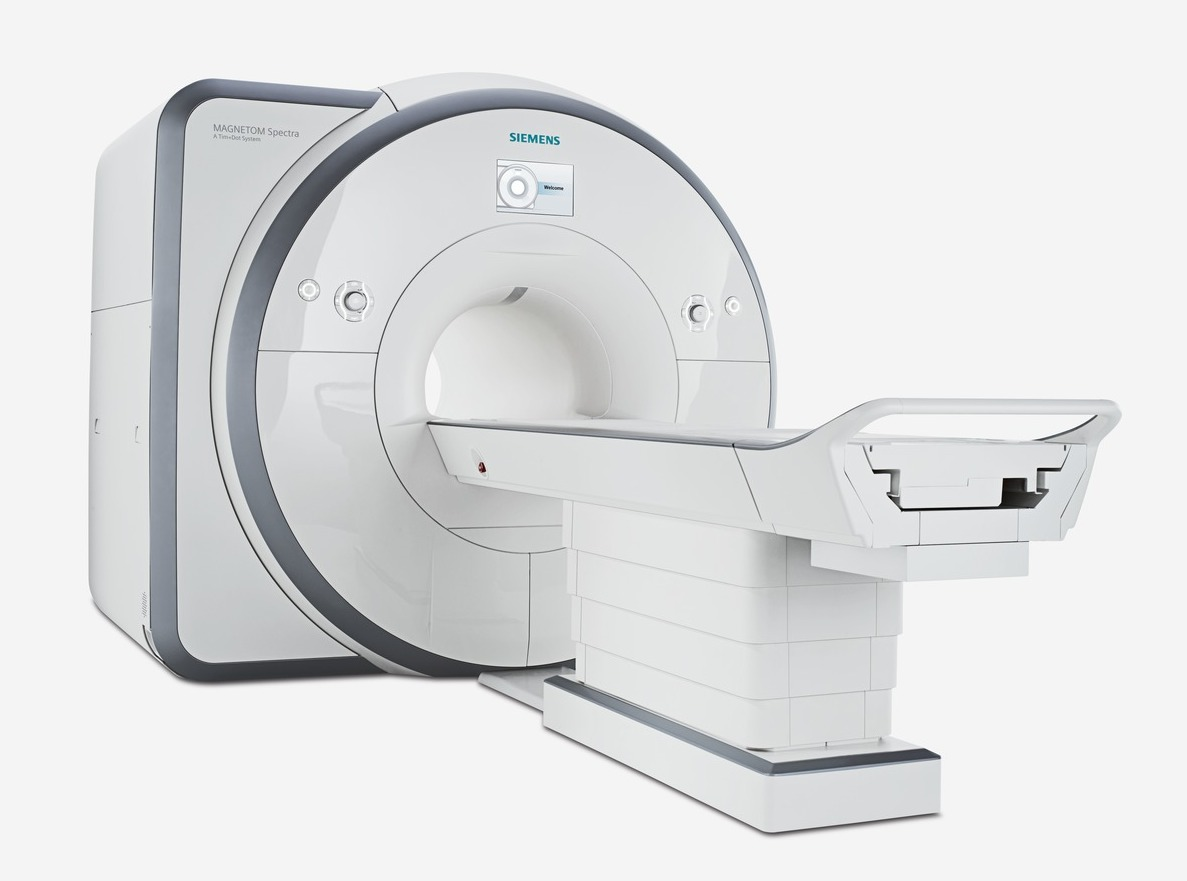
\includegraphics[height=0.9\textheight]{images/spectra}
    \end{center}
\end{frame}

\begin{frame}[c]{CT vs.~MRI}

    \begin{columns}[c,onlytextwidth]
        \column{0.47\textwidth}
        \centering{}
        \begin{block}{CT}
            \begin{itemize}
                \small
                \item High radiation dose
                \item 1 contrast: x-ray attenuation
                \item Good bone contrast
                \item Spatial resolution: 0.4\,mm
                \item Scan time: seconds
                \item Almost fixed image orientation
                      %\item Cost: High (\$85k - \$450k)
            \end{itemize}
        \end{block}%
        \column{0.5\textwidth}%
        \begin{block}{MRI}
            \centering{}
            \begin{itemize}
                \small
                \item No ionizing radiation
                \item Different types of contrast
                \item Good soft-tissue contrast
                \item Spatial resolution: 0.5 -- 3\,mm
                \item Scan time: minutes
                \item Arbitrary image orientation
                      %\item Cost: Very high (\$700k - \$1.5M)
            \end{itemize}
        \end{block}

    \end{columns}

\end{frame}
\begin{frame}[c]{CT vs.~MRI}
    \begin{figure}
        \centering
        \subcaptionbox{CT*}{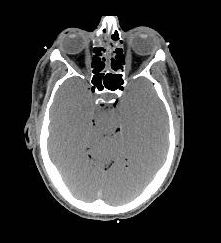
\includegraphics[height=3.3cm]{images/vhm-brainct}}
        \subcaptionbox{\longtime{}-weighted MRI}{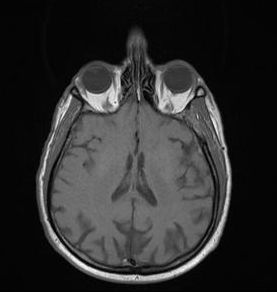
\includegraphics[height=3.3cm]{images/5009-dkfz-t1}}
        \subcaptionbox{\transtime{}-weighted MRI}{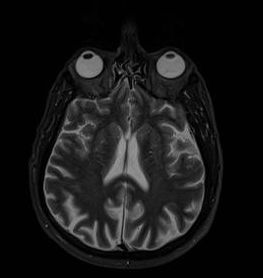
\includegraphics[height=3.3cm]{images/5009-dkfz-t2}}
    \end{figure}

    {\scriptsize *Source: Visible Human Project}
\end{frame}

% section introduction (end)



\section{Nuclear Magnetic Resonance (NMR)}% (fold)
\label{sec:nuclear_magnetic_resonance_nmr}

% [allowframebreaks] is not compatible with overlays -> do it manually :-(
\begin{frame}{Compass Needle Example I}

Behavior of a compass needle subjected to the earth's magnetic field

\begin{center}
\begingroup
\tikzset{every picture/.style={scale=0.9}}%
\only<1>{\tikzsetnextfilename{mr_compass_1}
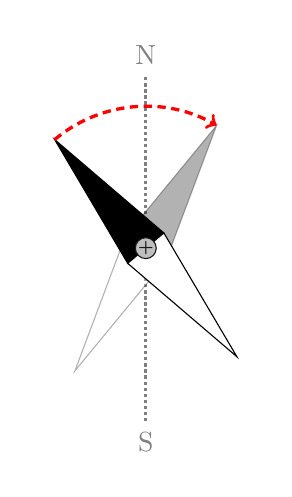
\begin{tikzpicture}
	\clip (-1.5, -2.8) rectangle (1.5, 2.8);
	\draw[gray, very thick, densely dotted] (0, -2.2) node [below] {S} -- (0, 2.2) node [above] {N};
	\begin{scope}[rotate=-30, opacity=0.3]
		\filldraw (-0.3, 0) -- (0.3, 0) -- (0, 1.8) -- cycle;
		\filldraw[fill=white] (-0.3, 0) -- (0.3, 0) -- (0, -1.8) -- cycle;
		\node[circle, inner sep=0pt, gray!20!black, draw=gray!20!black, fill=gray!50!white] at (0, 0) {{\tiny \textbf{+}}};
	\end{scope}
	\begin{scope}[rotate=40]
		\filldraw (-0.3, 0) -- (0.3, 0) -- (0, 1.8) -- cycle;
		\filldraw[fill=white] (-0.3, 0) -- (0.3, 0) -- (0, -1.8) -- cycle;
		\node[circle, inner sep=0pt, gray!20!black, draw=gray!20!black, fill=gray!50!white] at (0, 0) {{\tiny \textbf{+}}};
		\draw[very thick, densely dashed, red, ->] (0, 1.8) arc (90:20:1.8);
	\end{scope}
\end{tikzpicture}}%
\only<2>{\tikzsetnextfilename{mr_compass_2}
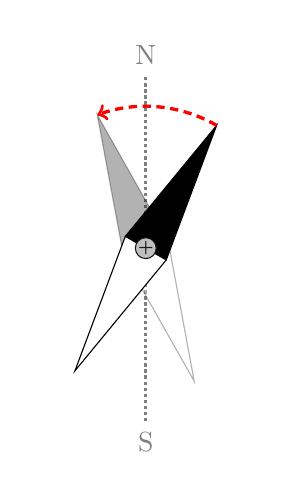
\begin{tikzpicture}
	\clip (-1.5, -2.8) rectangle (1.5, 2.8);
	\draw[gray, very thick, densely dotted] (0, -2.2) node [below] {S} -- (0, 2.2) node [above] {N};
	\begin{scope}[rotate=20, opacity=0.3]
		\filldraw (-0.3, 0) -- (0.3, 0) -- (0, 1.8) -- cycle;
		\filldraw[fill=white] (-0.3, 0) -- (0.3, 0) -- (0, -1.8) -- cycle;
		\node[circle, inner sep=0pt, gray!20!black, draw=gray!20!black, fill=gray!50!white] at (0, 0) {{\tiny \textbf{+}}};
	\end{scope}
	\begin{scope}[rotate=-30]
		\filldraw (-0.3, 0) -- (0.3, 0) -- (0, 1.8) -- cycle;
		\filldraw[fill=white] (-0.3, 0) -- (0.3, 0) -- (0, -1.8) -- cycle;
		\node[circle, inner sep=0pt, gray!20!black, draw=gray!20!black, fill=gray!50!white] at (0, 0) {{\tiny \textbf{+}}};
		\draw[very thick, densely dashed, red, ->] (0, 1.8) arc (90:140:1.8);
	\end{scope}
\end{tikzpicture}}%
\only<3>{\tikzsetnextfilename{mr_compass_3}
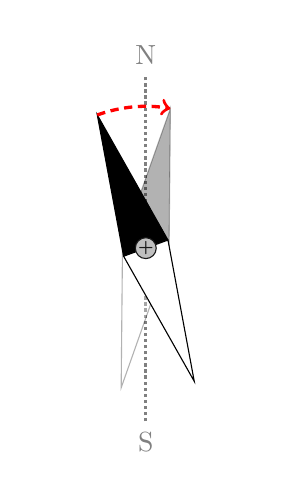
\begin{tikzpicture}
	\clip (-1.5, -2.8) rectangle (1.5, 2.8);
	\draw[gray, very thick, densely dotted] (0, -2.2) node [below] {S} -- (0, 2.2) node [above] {N};
	\begin{scope}[rotate=-10, opacity=0.3]
		\filldraw (-0.3, 0) -- (0.3, 0) -- (0, 1.8) -- cycle;
		\filldraw[fill=white] (-0.3, 0) -- (0.3, 0) -- (0, -1.8) -- cycle;
		\node[circle, inner sep=0pt, gray!20!black, draw=gray!20!black, fill=gray!50!white] at (0, 0) {{\tiny \textbf{+}}};
	\end{scope}
	\begin{scope}[rotate=20]
		\filldraw (-0.3, 0) -- (0.3, 0) -- (0, 1.8) -- cycle;
		\filldraw[fill=white] (-0.3, 0) -- (0.3, 0) -- (0, -1.8) -- cycle;
		\node[circle, inner sep=0pt, gray!20!black, draw=gray!20!black, fill=gray!50!white] at (0, 0) {{\tiny \textbf{+}}};
		\draw[very thick, densely dashed, red, ->] (0, 1.8) arc (90:60:1.8);
	\end{scope}
\end{tikzpicture}}%
\only<4>{\tikzsetnextfilename{mr_compass_4}
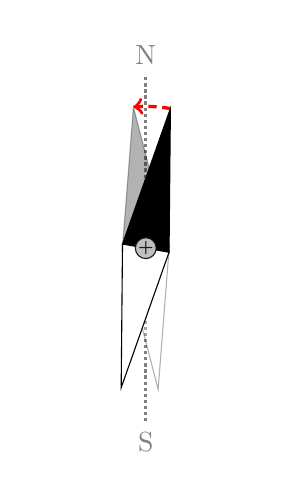
\begin{tikzpicture}
	\clip (-1.5, -2.8) rectangle (1.5, 2.8);
	\draw[gray, very thick, densely dotted] (0, -2.2) node [below] {S} -- (0, 2.2) node [above] {N};
	\begin{scope}[rotate=5, opacity=0.3]
		\filldraw (-0.3, 0) -- (0.3, 0) -- (0, 1.8) -- cycle;
		\filldraw[fill=white] (-0.3, 0) -- (0.3, 0) -- (0, -1.8) -- cycle;
		\node[circle, inner sep=0pt, gray!20!black, draw=gray!20!black, fill=gray!50!white] at (0, 0) {{\tiny \textbf{+}}};
	\end{scope}
	\begin{scope}[rotate=-10]
		\filldraw (-0.3, 0) -- (0.3, 0) -- (0, 1.8) -- cycle;
		\filldraw[fill=white] (-0.3, 0) -- (0.3, 0) -- (0, -1.8) -- cycle;
		\node[circle, inner sep=0pt, gray!20!black, draw=gray!20!black, fill=gray!50!white] at (0, 0) {{\tiny \textbf{+}}};
		\draw[very thick, densely dashed, red, ->] (0, 1.8) arc (90:105:1.8);
	\end{scope}
\end{tikzpicture}}%
\endgroup
\end{center}

\end{frame}

\begin{frame}{Compass Needle Example II}

    \begin{itemize}
        \item Oscillations ``through north'' until convergence
              \begin{itemize}
                  \item Amplitude of the oscillations decreases over time
                  \item Frequency \textbf{stays the same}
                  \item Frequency is determined by magnetic field strength and \\ properties of the needle material
              \end{itemize}
        \item Real compasses $\rightarrow$ dampening fluid
    \end{itemize}

\end{frame}

\begin{frame}{Compass Needle Example III}

    \begin{itemize}
        \item Radiofrequency (RF) wave $\sim$ time-varying magnetic field
        \item $\rightarrow$ Oscillating needle causes emission of RF waves with the \\ same frequency as the oscillation
        \item Can be measured with a receiver coil $\rightarrow$ current is induced
    \end{itemize}

    \begin{center}
        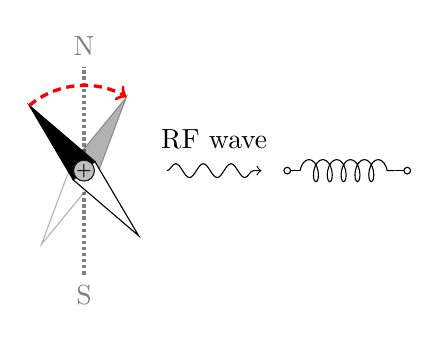
\begin{tikzpicture}[scale=0.6]
            \begin{scope}[xshift=-5ex]
                \draw[gray, very thick, densely dotted] (0, -2.2) node [below] {S} -- (0, 2.2) node [above] {N};
                \begin{scope}[rotate=-30, opacity=0.3]
                    \filldraw (-0.3, 0) -- (0.3, 0) -- (0, 1.8) -- cycle;
                    \filldraw[fill=white] (-0.3, 0) -- (0.3, 0) -- (0, -1.8) -- cycle;
                    \node[circle, inner sep=0pt, gray!20!black, draw=gray!20!black, fill=gray!50!white] at (0, 0) {{\tiny \textbf{+}}};
                \end{scope}
                \begin{scope}[rotate=40]
                    \filldraw (-0.3, 0) -- (0.3, 0) -- (0, 1.8) -- cycle;
                    \filldraw[fill=white] (-0.3, 0) -- (0.3, 0) -- (0, -1.8) -- cycle;
                    \node[circle, inner sep=0pt, gray!20!black, draw=gray!20!black, fill=gray!50!white] at (0, 0) {{\tiny \textbf{+}}};
                    \draw[very thick, densely dashed, red, ->] (0, 1.8) arc (90:20:1.8);
                \end{scope}
            \end{scope}

            \draw[decorate,decoration={snake},->] (1, 0) -- node [above=1ex] {RF wave} (3, 0);

            \begin{scope}[xshift=12ex]
                \draw[decorate,decoration={coil, amplitude=4pt,
                            segment length=5pt}] (2, 0) -- (4, 0);
                \draw (1.8, 0) -- (2, 0);
                \draw (4, 0) -- (4.2, 0);
                \draw (1.8, 0) ++(-2pt, 0) circle (2pt);
                \draw (4.2, 0) ++(2pt, 0) circle (2pt);
            \end{scope}
        \end{tikzpicture}
    \end{center}

\end{frame}

\begin{frame}{Compass Needle Example IV}

    \begin{itemize}
        \item Receiver coil can also be used as a sender by \\ applying an external current
        \item Emission of an RF wave at the oscillation frequency can \\ increase the amplitude of the oscillation
        \item We call this frequency the \textbf{resonance frequency} of the needle
    \end{itemize}

    \begin{center}
        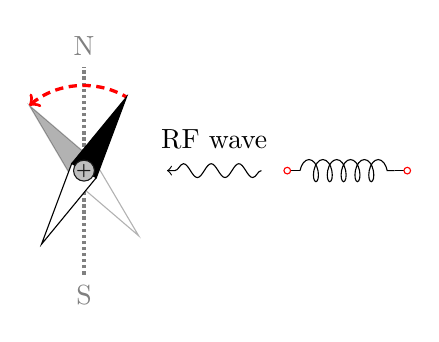
\begin{tikzpicture}[scale=0.6]
            \begin{scope}[xshift=-5ex]
                \draw[gray, very thick, densely dotted] (0, -2.2) node [below] {S} -- (0, 2.2) node [above] {N};
                \begin{scope}[rotate=40, opacity=0.3]
                    \filldraw (-0.3, 0) -- (0.3, 0) -- (0, 1.8) -- cycle;
                    \filldraw[fill=white] (-0.3, 0) -- (0.3, 0) -- (0, -1.8) -- cycle;
                    \node[circle, inner sep=0pt, gray!20!black, draw=gray!20!black, fill=gray!50!white] at (0, 0) {{\tiny \textbf{+}}};
                \end{scope}
                \begin{scope}[rotate=40]
                    \draw[very thick, densely dashed, red, <-] (0, 1.8) arc (90:20:1.8);
                \end{scope}
                \begin{scope}[rotate=-30]
                    \filldraw (-0.3, 0) -- (0.3, 0) -- (0, 1.8) -- cycle;
                    \filldraw[fill=white] (-0.3, 0) -- (0.3, 0) -- (0, -1.8) -- cycle;
                    \node[circle, inner sep=0pt, gray!20!black, draw=gray!20!black, fill=gray!50!white] at (0, 0) {{\tiny \textbf{+}}};
                \end{scope}
            \end{scope}

            \draw[decorate,decoration={snake,pre length=1mm},<-] (1, 0) -- node [above=1ex] {RF wave} (3, 0);

            \begin{scope}[xshift=12ex]
                \draw[decorate,decoration={coil, amplitude=4pt,
                            segment length=5pt}] (2, 0) -- (4, 0);
                \draw (1.8, 0) -- (2, 0);
                \draw (4, 0) -- (4.2, 0);
                \draw[red] (1.8, 0) ++(-2pt, 0) circle (2pt);
                \draw[red] (4.2, 0) ++(2pt, 0) circle (2pt);
            \end{scope}
        \end{tikzpicture}
    \end{center}

\end{frame}

\begin{frame}{Compass Needle Example V}

    \begin{center}
        \url{http://drcmr.dk/JavaCompass/}
    \end{center}
\end{frame}



\subsection{Genesis of the Resonance Effect} % (fold)
\label{sub:genesis_of_the_resonance_effect}

\begin{frame}{Magnetic Field}

    \begin{itemize}
        \item Can be produced by electric currents and magnetic materials
        \item Like a vector field, it is specified by an orientation and magnitude
        \item The field strength of magnets for imaging is given in \emph{teslas}
              \begin{itemize}
                  \item Earth's magnetic field: $6 \cdot 10^{-6}$ T
                  \item Typical MRI field strength: 1.5 or 3 T
              \end{itemize}
    \end{itemize}

    \begin{figure}
        \centering
        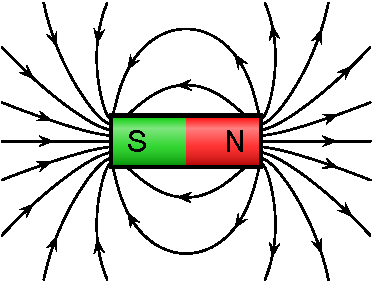
\includegraphics[height=2.5cm]{images/magnetic_field.pdf}
    \end{figure}

\end{frame}

\begin{frame}{Hydrogen Nuclei}
    \framesubtitle{"Magnetic needles" in the human body}

    \begin{figure}
        \centering
        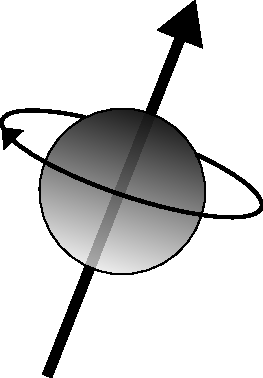
\includegraphics[height=2.5cm]{images/nuclear_spin.pdf}
    \end{figure}

    \begin{itemize}
        \item Hydrogen nuclei (\hydrogen) are used for MR imaging
              \begin{itemize}
                  \item Vast amount in the human body ($\sim 10^{27}$ nuclei)
                  \item Intrinsic property: magnetic spin around their rotation axis
              \end{itemize}
    \end{itemize}
\end{frame}

\begin{frame}{Random Spins}
    %
    \begin{itemize}
        \item Hydrogen nuclei are randomly interacting within the body
              \begin{itemize}
                  \item Their spin axes point in random directions
                  \item $\rightarrow$ The net magnetization \magn, which is the sum of all spin axes,\\ is roughly zero
              \end{itemize}
    \end{itemize}
    %
    \begin{figure}
        \centering
        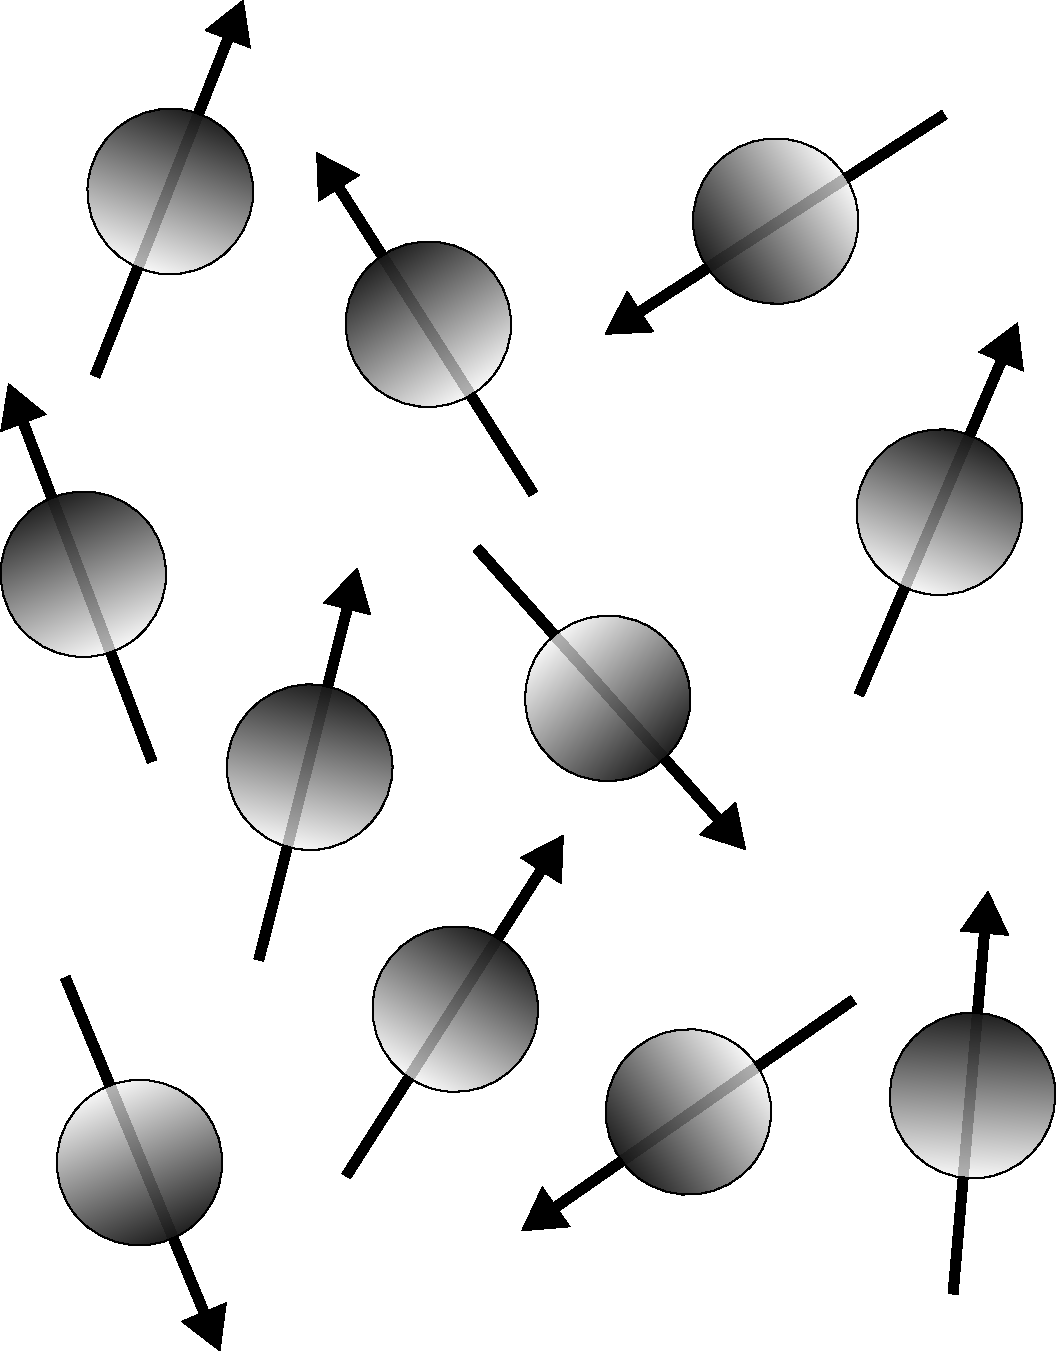
\includegraphics[height=3.8cm]{images/random_spins.pdf}
    \end{figure}

\end{frame}


\begin{frame}{Aligned Spins}

    \begin{itemize}
        \item A strong magnet can make the axes of nuclei align towards the magnetic field direction \B0
              \begin{itemize}
                  \item The spins partially align and tend to point in one direction
                  \item $\rightarrow$ Net magnetization \magn~is greater zero
              \end{itemize}
    \end{itemize}

    \begin{figure}
        \centering
        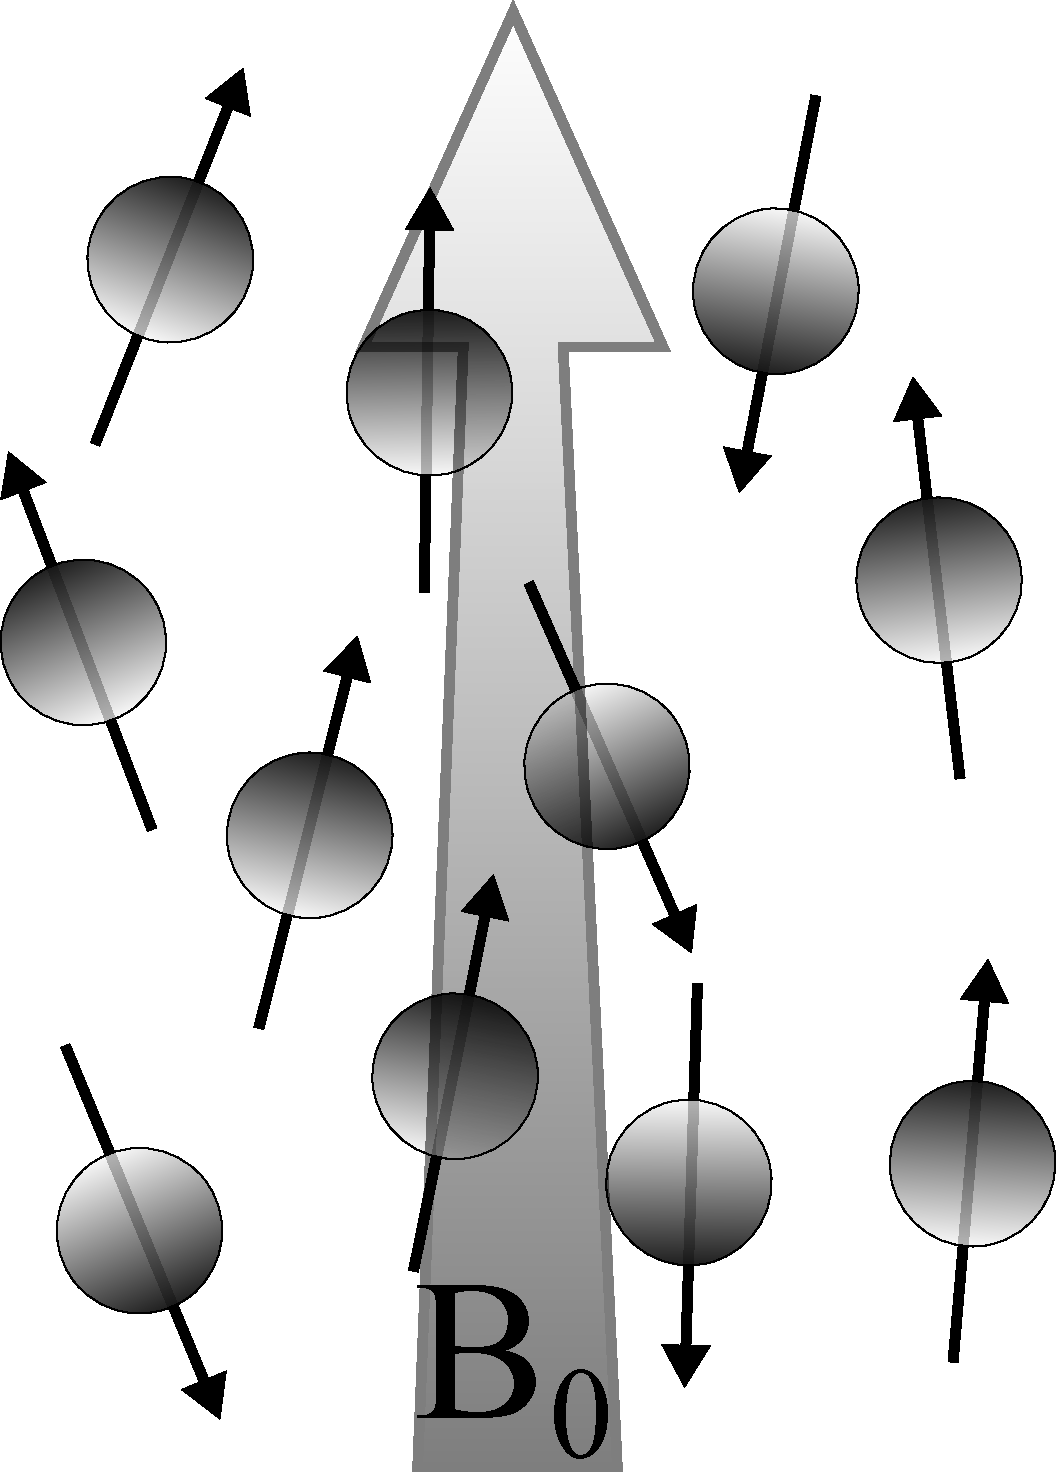
\includegraphics[height=3.8cm]{images/aligned_spins.pdf}
    \end{figure}
    
\end{frame}

\begin{frame}{Precession}
    \framesubtitle{Net magnetization gyrates like a spin top}

    \begin{figure}
        \centering
        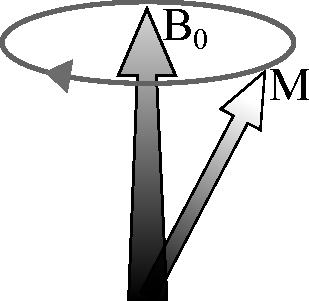
\includegraphics[height=3cm]{images/precession.pdf}
    \end{figure}



    \begin{itemize}
        \item 	\magn~rotates (precesses) around an activated magnetic field \B0
        \item The net magnetization vector gradually aligns with \B0
        \item Equivalent to the oscillation of the compass needle
    \end{itemize}

\end{frame}

\begin{frame}{Larmor Frequency}

    \begin{itemize}
        \item The Larmor or resonance frequency $\larmorfreq = \gamma \cdot \Vert \B{0} \Vert$, defines the frequency of this precession
        \item Gyromagnetic ratio $\gamma$ is $42.576\,\mathsf{MHz/T}$ for hydrogen nuclei
        \item Inside a 1.5 T magnet, \magn~precesses with about $\larmorfreq = 64\,\mathsf{MHz}$
    \end{itemize}
\end{frame}

\begin{frame}{Excitation}
    \framesubtitle{Pushing the magnetization out of its stable position}

    \begin{itemize}
        \item Analogously to the compass example, \magn~can be pushed \\out of its stable position
              %		\begin{itemize}
        \item Applying RF pulses orthogonal to \B0 with the resonance frequency of \magn~introduces a weaker field \B1
        \item $\rightarrow$ \magn~both precesses around \B0 and \B1 like a falling spin top
              %	\item Upon stopping the RF pulses, \magn reverses its trajectory and produces a current
              %		\end{itemize}
    \end{itemize}
\end{frame}

\begin{frame}{Excitation cont.}

    \begin{center}
        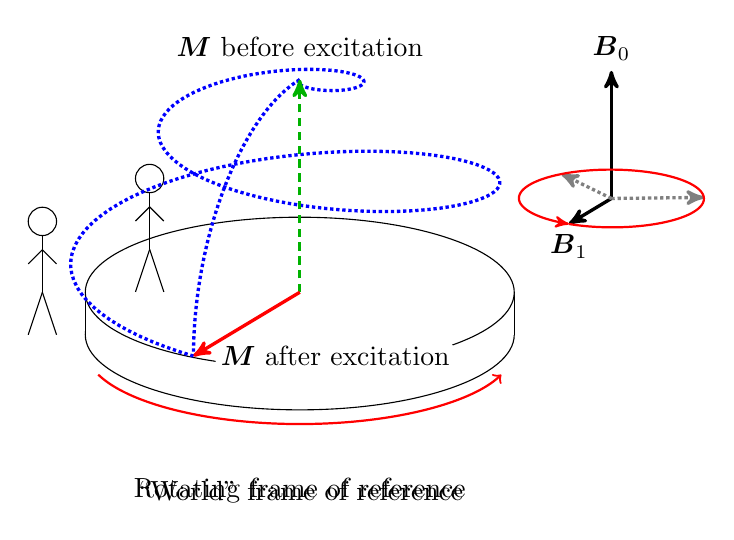
\begin{tikzpicture}[scale=1.8]
            %\draw[draw=none] (-2.5,-1.4) rectangle (2.7,2.5);

            \draw (0, -0.3) ellipse (10ex and 3.5ex);
            \fill[white] (-10ex, 0) -- (10ex, 0) -- (10ex, -0.3) -- (-10ex, -0.3) -- cycle;
            \draw (-10ex, 0) -- (-10ex, -0.3);
            \draw ( 10ex, 0) -- ( 10ex, -0.3);
            \draw[fill=white] (0, 0) ellipse (10ex and 3.5ex);

            \draw[red, thick, ->] (0, -0.4) + (200:10ex and 3.5ex) arc (200:340:10ex and 3.5ex);

            % Stick figure
            \visible<1>{\draw (-12ex, 0.5) circle (0.1);
                \draw (-12ex, 0.4) -- (-12ex, 0);
                \draw (-12ex, 0.3) -- ++(0.1, -0.1);
                \draw (-12ex, 0.3) -- ++(-0.1, -0.1);
                \draw (-12ex, 0) -- ++(0.1, -0.3);
                \draw (-12ex, 0) -- ++(-0.1, -0.3);}

            \visible<1>{\draw (0, -1.4) node {``World'' frame of reference};}
            \visible<2>{\draw (0, -1.4) node {Rotating frame of reference};}

            \visible<2>{
                \begin{scope}[xshift=5ex, yshift=2ex]
                    \draw (-12ex, 0.5) circle (0.1);
                    \draw (-12ex, 0.4) -- (-12ex, 0);
                    \draw (-12ex, 0.3) -- ++(0.1, -0.1);
                    \draw (-12ex, 0.3) -- ++(-0.1, -0.1);
                    \draw (-12ex, 0) -- ++(0.1, -0.3);
                    \draw (-12ex, 0) -- ++(-0.1, -0.3);
                \end{scope}
            }

            \begin{scope}[%overlay,
                    x  = {(-0.5cm,-0.3cm)},
                    y  = {(0.9659cm,-0.15882cm)},
                    z  = {(0cm,1cm)},
                    scale = 1.5,
                    >=stealth']
                %\draw[->] (-1.2, 0, 0) -- (1.2, 0, 0) node [below left] {$x$};
                %\draw[->] (0, -1.2, 0) -- (0, 1.2, 0) node [right] {$y$};
                %\draw[->] (0, 0, -0.2) -- (0, 0, 1) node [above] {$z$};

                %\draw[red, thick, ->] (0, -0.4) [partial ellipse=200:340:10ex and 3.5ex];
                \draw[very thick,->] (-1,1,0.3) -- (-1,1,0.9) node [above] {\B0};
                \draw[very thick,->] (-1,1,0.3) -- (-0.6,1,0.3) node [below] {\B1};
                \visible<1>{
                    \draw[very thick,gray,densely dotted,->] (-1,1,0.3) -- (-1.2000,  1.3464,  0.3000);
                    \draw[very thick,gray, densely dotted,->] (-1,1,0.3) -- (-1.2000,  0.6536,  0.3000);

                    \draw[red, thick, ->] (-0.6000,  1.0000,  0.3000)
                    -- (-0.6001,  1.0070,  0.3000)
                    -- (-0.6002,  1.0140,  0.3000)
                    -- (-0.6005,  1.0209,  0.3000)
                    -- (-0.6010,  1.0279,  0.3000)
                    -- (-0.6015,  1.0349,  0.3000)
                    -- (-0.6022,  1.0418,  0.3000)
                    -- (-0.6030,  1.0487,  0.3000)
                    -- (-0.6039,  1.0557,  0.3000)
                    -- (-0.6049,  1.0626,  0.3000)
                    -- (-0.6061,  1.0695,  0.3000)
                    -- (-0.6073,  1.0763,  0.3000)
                    -- (-0.6087,  1.0832,  0.3000)
                    -- (-0.6103,  1.0900,  0.3000)
                    -- (-0.6119,  1.0968,  0.3000)
                    -- (-0.6136,  1.1035,  0.3000)
                    -- (-0.6155,  1.1103,  0.3000)
                    -- (-0.6175,  1.1169,  0.3000)
                    -- (-0.6196,  1.1236,  0.3000)
                    -- (-0.6218,  1.1302,  0.3000)
                    -- (-0.6241,  1.1368,  0.3000)
                    -- (-0.6266,  1.1433,  0.3000)
                    -- (-0.6291,  1.1498,  0.3000)
                    -- (-0.6318,  1.1563,  0.3000)
                    -- (-0.6346,  1.1627,  0.3000)
                    -- (-0.6375,  1.1690,  0.3000)
                    -- (-0.6405,  1.1753,  0.3000)
                    -- (-0.6436,  1.1816,  0.3000)
                    -- (-0.6468,  1.1878,  0.3000)
                    -- (-0.6502,  1.1939,  0.3000)
                    -- (-0.6536,  1.2000,  0.3000)
                    -- (-0.6571,  1.2060,  0.3000)
                    -- (-0.6608,  1.2120,  0.3000)
                    -- (-0.6645,  1.2179,  0.3000)
                    -- (-0.6684,  1.2237,  0.3000)
                    -- (-0.6723,  1.2294,  0.3000)
                    -- (-0.6764,  1.2351,  0.3000)
                    -- (-0.6805,  1.2407,  0.3000)
                    -- (-0.6848,  1.2463,  0.3000)
                    -- (-0.6891,  1.2517,  0.3000)
                    -- (-0.6936,  1.2571,  0.3000)
                    -- (-0.6981,  1.2624,  0.3000)
                    -- (-0.7027,  1.2677,  0.3000)
                    -- (-0.7075,  1.2728,  0.3000)
                    -- (-0.7123,  1.2779,  0.3000)
                    -- (-0.7172,  1.2828,  0.3000)
                    -- (-0.7221,  1.2877,  0.3000)
                    -- (-0.7272,  1.2925,  0.3000)
                    -- (-0.7323,  1.2973,  0.3000)
                    -- (-0.7376,  1.3019,  0.3000)
                    -- (-0.7429,  1.3064,  0.3000)
                    -- (-0.7483,  1.3109,  0.3000)
                    -- (-0.7537,  1.3152,  0.3000)
                    -- (-0.7593,  1.3195,  0.3000)
                    -- (-0.7649,  1.3236,  0.3000)
                    -- (-0.7706,  1.3277,  0.3000)
                    -- (-0.7763,  1.3316,  0.3000)
                    -- (-0.7821,  1.3355,  0.3000)
                    -- (-0.7880,  1.3392,  0.3000)
                    -- (-0.7940,  1.3429,  0.3000)
                    -- (-0.8000,  1.3464,  0.3000)
                    -- (-0.8061,  1.3498,  0.3000)
                    -- (-0.8122,  1.3532,  0.3000)
                    -- (-0.8184,  1.3564,  0.3000)
                    -- (-0.8247,  1.3595,  0.3000)
                    -- (-0.8310,  1.3625,  0.3000)
                    -- (-0.8373,  1.3654,  0.3000)
                    -- (-0.8437,  1.3682,  0.3000)
                    -- (-0.8502,  1.3709,  0.3000)
                    -- (-0.8567,  1.3734,  0.3000)
                    -- (-0.8632,  1.3759,  0.3000)
                    -- (-0.8698,  1.3782,  0.3000)
                    -- (-0.8764,  1.3804,  0.3000)
                    -- (-0.8831,  1.3825,  0.3000)
                    -- (-0.8897,  1.3845,  0.3000)
                    -- (-0.8965,  1.3864,  0.3000)
                    -- (-0.9032,  1.3881,  0.3000)
                    -- (-0.9100,  1.3897,  0.3000)
                    -- (-0.9168,  1.3913,  0.3000)
                    -- (-0.9237,  1.3927,  0.3000)
                    -- (-0.9305,  1.3939,  0.3000)
                    -- (-0.9374,  1.3951,  0.3000)
                    -- (-0.9443,  1.3961,  0.3000)
                    -- (-0.9513,  1.3970,  0.3000)
                    -- (-0.9582,  1.3978,  0.3000)
                    -- (-0.9651,  1.3985,  0.3000)
                    -- (-0.9721,  1.3990,  0.3000)
                    -- (-0.9791,  1.3995,  0.3000)
                    -- (-0.9860,  1.3998,  0.3000)
                    -- (-0.9930,  1.3999,  0.3000)
                    -- (-1.0000,  1.4000,  0.3000)
                    -- (-1.0070,  1.3999,  0.3000)
                    -- (-1.0140,  1.3998,  0.3000)
                    -- (-1.0209,  1.3995,  0.3000)
                    -- (-1.0279,  1.3990,  0.3000)
                    -- (-1.0349,  1.3985,  0.3000)
                    -- (-1.0418,  1.3978,  0.3000)
                    -- (-1.0487,  1.3970,  0.3000)
                    -- (-1.0557,  1.3961,  0.3000)
                    -- (-1.0626,  1.3951,  0.3000)
                    -- (-1.0695,  1.3939,  0.3000)
                    -- (-1.0763,  1.3927,  0.3000)
                    -- (-1.0832,  1.3913,  0.3000)
                    -- (-1.0900,  1.3897,  0.3000)
                    -- (-1.0968,  1.3881,  0.3000)
                    -- (-1.1035,  1.3864,  0.3000)
                    -- (-1.1103,  1.3845,  0.3000)
                    -- (-1.1169,  1.3825,  0.3000)
                    -- (-1.1236,  1.3804,  0.3000)
                    -- (-1.1302,  1.3782,  0.3000)
                    -- (-1.1368,  1.3759,  0.3000)
                    -- (-1.1433,  1.3734,  0.3000)
                    -- (-1.1498,  1.3709,  0.3000)
                    -- (-1.1563,  1.3682,  0.3000)
                    -- (-1.1627,  1.3654,  0.3000)
                    -- (-1.1690,  1.3625,  0.3000)
                    -- (-1.1753,  1.3595,  0.3000)
                    -- (-1.1816,  1.3564,  0.3000)
                    -- (-1.1878,  1.3532,  0.3000)
                    -- (-1.1939,  1.3498,  0.3000)
                    -- (-1.2000,  1.3464,  0.3000)
                    -- (-1.2060,  1.3429,  0.3000)
                    -- (-1.2120,  1.3392,  0.3000)
                    -- (-1.2179,  1.3355,  0.3000)
                    -- (-1.2237,  1.3316,  0.3000)
                    -- (-1.2294,  1.3277,  0.3000)
                    -- (-1.2351,  1.3236,  0.3000)
                    -- (-1.2407,  1.3195,  0.3000)
                    -- (-1.2463,  1.3152,  0.3000)
                    -- (-1.2517,  1.3109,  0.3000)
                    -- (-1.2571,  1.3064,  0.3000)
                    -- (-1.2624,  1.3019,  0.3000)
                    -- (-1.2677,  1.2973,  0.3000)
                    -- (-1.2728,  1.2925,  0.3000)
                    -- (-1.2779,  1.2877,  0.3000)
                    -- (-1.2828,  1.2828,  0.3000)
                    -- (-1.2877,  1.2779,  0.3000)
                    -- (-1.2925,  1.2728,  0.3000)
                    -- (-1.2973,  1.2677,  0.3000)
                    -- (-1.3019,  1.2624,  0.3000)
                    -- (-1.3064,  1.2571,  0.3000)
                    -- (-1.3109,  1.2517,  0.3000)
                    -- (-1.3152,  1.2463,  0.3000)
                    -- (-1.3195,  1.2407,  0.3000)
                    -- (-1.3236,  1.2351,  0.3000)
                    -- (-1.3277,  1.2294,  0.3000)
                    -- (-1.3316,  1.2237,  0.3000)
                    -- (-1.3355,  1.2179,  0.3000)
                    -- (-1.3392,  1.2120,  0.3000)
                    -- (-1.3429,  1.2060,  0.3000)
                    -- (-1.3464,  1.2000,  0.3000)
                    -- (-1.3498,  1.1939,  0.3000)
                    -- (-1.3532,  1.1878,  0.3000)
                    -- (-1.3564,  1.1816,  0.3000)
                    -- (-1.3595,  1.1753,  0.3000)
                    -- (-1.3625,  1.1690,  0.3000)
                    -- (-1.3654,  1.1627,  0.3000)
                    -- (-1.3682,  1.1563,  0.3000)
                    -- (-1.3709,  1.1498,  0.3000)
                    -- (-1.3734,  1.1433,  0.3000)
                    -- (-1.3759,  1.1368,  0.3000)
                    -- (-1.3782,  1.1302,  0.3000)
                    -- (-1.3804,  1.1236,  0.3000)
                    -- (-1.3825,  1.1169,  0.3000)
                    -- (-1.3845,  1.1103,  0.3000)
                    -- (-1.3864,  1.1035,  0.3000)
                    -- (-1.3881,  1.0968,  0.3000)
                    -- (-1.3897,  1.0900,  0.3000)
                    -- (-1.3913,  1.0832,  0.3000)
                    -- (-1.3927,  1.0763,  0.3000)
                    -- (-1.3939,  1.0695,  0.3000)
                    -- (-1.3951,  1.0626,  0.3000)
                    -- (-1.3961,  1.0557,  0.3000)
                    -- (-1.3970,  1.0487,  0.3000)
                    -- (-1.3978,  1.0418,  0.3000)
                    -- (-1.3985,  1.0349,  0.3000)
                    -- (-1.3990,  1.0279,  0.3000)
                    -- (-1.3995,  1.0209,  0.3000)
                    -- (-1.3998,  1.0140,  0.3000)
                    -- (-1.3999,  1.0070,  0.3000)
                    -- (-1.4000,  1.0000,  0.3000)
                    -- (-1.3999,  0.9930,  0.3000)
                    -- (-1.3998,  0.9860,  0.3000)
                    -- (-1.3995,  0.9791,  0.3000)
                    -- (-1.3990,  0.9721,  0.3000)
                    -- (-1.3985,  0.9651,  0.3000)
                    -- (-1.3978,  0.9582,  0.3000)
                    -- (-1.3970,  0.9513,  0.3000)
                    -- (-1.3961,  0.9443,  0.3000)
                    -- (-1.3951,  0.9374,  0.3000)
                    -- (-1.3939,  0.9305,  0.3000)
                    -- (-1.3927,  0.9237,  0.3000)
                    -- (-1.3913,  0.9168,  0.3000)
                    -- (-1.3897,  0.9100,  0.3000)
                    -- (-1.3881,  0.9032,  0.3000)
                    -- (-1.3864,  0.8965,  0.3000)
                    -- (-1.3845,  0.8897,  0.3000)
                    -- (-1.3825,  0.8831,  0.3000)
                    -- (-1.3804,  0.8764,  0.3000)
                    -- (-1.3782,  0.8698,  0.3000)
                    -- (-1.3759,  0.8632,  0.3000)
                    -- (-1.3734,  0.8567,  0.3000)
                    -- (-1.3709,  0.8502,  0.3000)
                    -- (-1.3682,  0.8437,  0.3000)
                    -- (-1.3654,  0.8373,  0.3000)
                    -- (-1.3625,  0.8310,  0.3000)
                    -- (-1.3595,  0.8247,  0.3000)
                    -- (-1.3564,  0.8184,  0.3000)
                    -- (-1.3532,  0.8122,  0.3000)
                    -- (-1.3498,  0.8061,  0.3000)
                    -- (-1.3464,  0.8000,  0.3000)
                    -- (-1.3429,  0.7940,  0.3000)
                    -- (-1.3392,  0.7880,  0.3000)
                    -- (-1.3355,  0.7821,  0.3000)
                    -- (-1.3316,  0.7763,  0.3000)
                    -- (-1.3277,  0.7706,  0.3000)
                    -- (-1.3236,  0.7649,  0.3000)
                    -- (-1.3195,  0.7593,  0.3000)
                    -- (-1.3152,  0.7537,  0.3000)
                    -- (-1.3109,  0.7483,  0.3000)
                    -- (-1.3064,  0.7429,  0.3000)
                    -- (-1.3019,  0.7376,  0.3000)
                    -- (-1.2973,  0.7323,  0.3000)
                    -- (-1.2925,  0.7272,  0.3000)
                    -- (-1.2877,  0.7221,  0.3000)
                    -- (-1.2828,  0.7172,  0.3000)
                    -- (-1.2779,  0.7123,  0.3000)
                    -- (-1.2728,  0.7075,  0.3000)
                    -- (-1.2677,  0.7027,  0.3000)
                    -- (-1.2624,  0.6981,  0.3000)
                    -- (-1.2571,  0.6936,  0.3000)
                    -- (-1.2517,  0.6891,  0.3000)
                    -- (-1.2463,  0.6848,  0.3000)
                    -- (-1.2407,  0.6805,  0.3000)
                    -- (-1.2351,  0.6764,  0.3000)
                    -- (-1.2294,  0.6723,  0.3000)
                    -- (-1.2237,  0.6684,  0.3000)
                    -- (-1.2179,  0.6645,  0.3000)
                    -- (-1.2120,  0.6608,  0.3000)
                    -- (-1.2060,  0.6571,  0.3000)
                    -- (-1.2000,  0.6536,  0.3000)
                    -- (-1.1939,  0.6502,  0.3000)
                    -- (-1.1878,  0.6468,  0.3000)
                    -- (-1.1816,  0.6436,  0.3000)
                    -- (-1.1753,  0.6405,  0.3000)
                    -- (-1.1690,  0.6375,  0.3000)
                    -- (-1.1627,  0.6346,  0.3000)
                    -- (-1.1563,  0.6318,  0.3000)
                    -- (-1.1498,  0.6291,  0.3000)
                    -- (-1.1433,  0.6266,  0.3000)
                    -- (-1.1368,  0.6241,  0.3000)
                    -- (-1.1302,  0.6218,  0.3000)
                    -- (-1.1236,  0.6196,  0.3000)
                    -- (-1.1169,  0.6175,  0.3000)
                    -- (-1.1103,  0.6155,  0.3000)
                    -- (-1.1035,  0.6136,  0.3000)
                    -- (-1.0968,  0.6119,  0.3000)
                    -- (-1.0900,  0.6103,  0.3000)
                    -- (-1.0832,  0.6087,  0.3000)
                    -- (-1.0763,  0.6073,  0.3000)
                    -- (-1.0695,  0.6061,  0.3000)
                    -- (-1.0626,  0.6049,  0.3000)
                    -- (-1.0557,  0.6039,  0.3000)
                    -- (-1.0487,  0.6030,  0.3000)
                    -- (-1.0418,  0.6022,  0.3000)
                    -- (-1.0349,  0.6015,  0.3000)
                    -- (-1.0279,  0.6010,  0.3000)
                    -- (-1.0209,  0.6005,  0.3000)
                    -- (-1.0140,  0.6002,  0.3000)
                    -- (-1.0070,  0.6001,  0.3000)
                    -- (-1.0000,  0.6000,  0.3000)
                    -- (-0.9930,  0.6001,  0.3000)
                    -- (-0.9860,  0.6002,  0.3000)
                    -- (-0.9791,  0.6005,  0.3000)
                    -- (-0.9721,  0.6010,  0.3000)
                    -- (-0.9651,  0.6015,  0.3000)
                    -- (-0.9582,  0.6022,  0.3000)
                    -- (-0.9513,  0.6030,  0.3000)
                    -- (-0.9443,  0.6039,  0.3000)
                    -- (-0.9374,  0.6049,  0.3000)
                    -- (-0.9305,  0.6061,  0.3000)
                    -- (-0.9237,  0.6073,  0.3000)
                    -- (-0.9168,  0.6087,  0.3000)
                    -- (-0.9100,  0.6103,  0.3000)
                    -- (-0.9032,  0.6119,  0.3000)
                    -- (-0.8965,  0.6136,  0.3000)
                    -- (-0.8897,  0.6155,  0.3000)
                    -- (-0.8831,  0.6175,  0.3000)
                    -- (-0.8764,  0.6196,  0.3000)
                    -- (-0.8698,  0.6218,  0.3000)
                    -- (-0.8632,  0.6241,  0.3000)
                    -- (-0.8567,  0.6266,  0.3000)
                    -- (-0.8502,  0.6291,  0.3000)
                    -- (-0.8437,  0.6318,  0.3000)
                    -- (-0.8373,  0.6346,  0.3000)
                    -- (-0.8310,  0.6375,  0.3000)
                    -- (-0.8247,  0.6405,  0.3000)
                    -- (-0.8184,  0.6436,  0.3000)
                    -- (-0.8122,  0.6468,  0.3000)
                    -- (-0.8061,  0.6502,  0.3000)
                    -- (-0.8000,  0.6536,  0.3000)
                    -- (-0.7940,  0.6571,  0.3000)
                    -- (-0.7880,  0.6608,  0.3000)
                    -- (-0.7821,  0.6645,  0.3000)
                    -- (-0.7763,  0.6684,  0.3000)
                    -- (-0.7706,  0.6723,  0.3000)
                    -- (-0.7649,  0.6764,  0.3000)
                    -- (-0.7593,  0.6805,  0.3000)
                    -- (-0.7537,  0.6848,  0.3000)
                    -- (-0.7483,  0.6891,  0.3000)
                    -- (-0.7429,  0.6936,  0.3000)
                    -- (-0.7376,  0.6981,  0.3000)
                    -- (-0.7323,  0.7027,  0.3000)
                    -- (-0.7272,  0.7075,  0.3000)
                    -- (-0.7221,  0.7123,  0.3000)
                    -- (-0.7172,  0.7172,  0.3000)
                    -- (-0.7123,  0.7221,  0.3000)
                    -- (-0.7075,  0.7272,  0.3000)
                    -- (-0.7027,  0.7323,  0.3000)
                    -- (-0.6981,  0.7376,  0.3000)
                    -- (-0.6936,  0.7429,  0.3000)
                    -- (-0.6891,  0.7483,  0.3000)
                    -- (-0.6848,  0.7537,  0.3000)
                    -- (-0.6805,  0.7593,  0.3000)
                    -- (-0.6764,  0.7649,  0.3000)
                    -- (-0.6723,  0.7706,  0.3000)
                    -- (-0.6684,  0.7763,  0.3000)
                    -- (-0.6645,  0.7821,  0.3000)
                    -- (-0.6608,  0.7880,  0.3000)
                    -- (-0.6571,  0.7940,  0.3000)
                    -- (-0.6536,  0.8000,  0.3000)
                    -- (-0.6502,  0.8061,  0.3000)
                    -- (-0.6468,  0.8122,  0.3000)
                    -- (-0.6436,  0.8184,  0.3000)
                    -- (-0.6405,  0.8247,  0.3000)
                    -- (-0.6375,  0.8310,  0.3000)
                    -- (-0.6346,  0.8373,  0.3000)
                    -- (-0.6318,  0.8437,  0.3000)
                    -- (-0.6291,  0.8502,  0.3000)
                    -- (-0.6266,  0.8567,  0.3000)
                    -- (-0.6241,  0.8632,  0.3000)
                    -- (-0.6218,  0.8698,  0.3000)
                    -- (-0.6196,  0.8764,  0.3000)
                    -- (-0.6175,  0.8831,  0.3000)
                    -- (-0.6155,  0.8897,  0.3000)
                    -- (-0.6136,  0.8965,  0.3000)
                    -- (-0.6119,  0.9032,  0.3000)
                    -- (-0.6103,  0.9100,  0.3000)
                    -- (-0.6087,  0.9168,  0.3000)
                    -- (-0.6073,  0.9237,  0.3000)
                    -- (-0.6061,  0.9305,  0.3000)
                    -- (-0.6049,  0.9374,  0.3000)
                    -- (-0.6039,  0.9443,  0.3000)
                    -- (-0.6030,  0.9513,  0.3000)
                    -- (-0.6022,  0.9582,  0.3000)
                    -- (-0.6015,  0.9651,  0.3000)
                    -- (-0.6010,  0.9721,  0.3000)
                    -- (-0.6005,  0.9791,  0.3000)
                    -- (-0.6002,  0.9860,  0.3000)
                    -- (-0.6001,  0.9930,  0.3000)
                    -- (-0.6000,  1.0000,  0.3000);}

                \visible<1>{\draw[blue, very thick, densely dotted] ( 0.0000,  0.0000,  1.0000)
                    -- ( 0.0087,  0.0006,  1.0000)
                    -- ( 0.0173,  0.0024,  0.9998)
                    -- ( 0.0256,  0.0054,  0.9997)
                    -- ( 0.0335,  0.0096,  0.9994)
                    -- ( 0.0410,  0.0149,  0.9990)
                    -- ( 0.0478,  0.0213,  0.9986)
                    -- ( 0.0539,  0.0287,  0.9981)
                    -- ( 0.0592,  0.0370,  0.9976)
                    -- ( 0.0635,  0.0461,  0.9969)
                    -- ( 0.0668,  0.0560,  0.9962)
                    -- ( 0.0689,  0.0666,  0.9954)
                    -- ( 0.0699,  0.0777,  0.9945)
                    -- ( 0.0697,  0.0892,  0.9936)
                    -- ( 0.0681,  0.1010,  0.9925)
                    -- ( 0.0653,  0.1130,  0.9914)
                    -- ( 0.0610,  0.1251,  0.9903)
                    -- ( 0.0554,  0.1370,  0.9890)
                    -- ( 0.0483,  0.1488,  0.9877)
                    -- ( 0.0399,  0.1601,  0.9863)
                    -- ( 0.0302,  0.1710,  0.9848)
                    -- ( 0.0190,  0.1812,  0.9833)
                    -- ( 0.0067,  0.1907,  0.9816)
                    -- (-0.0070,  0.1992,  0.9799)
                    -- (-0.0217,  0.2068,  0.9781)
                    -- (-0.0376,  0.2132,  0.9763)
                    -- (-0.0544,  0.2183,  0.9744)
                    -- (-0.0721,  0.2220,  0.9724)
                    -- (-0.0906,  0.2243,  0.9703)
                    -- (-0.1098,  0.2250,  0.9681)
                    -- (-0.1294,  0.2241,  0.9659)
                    -- (-0.1494,  0.2216,  0.9636)
                    -- (-0.1697,  0.2172,  0.9613)
                    -- (-0.1900,  0.2111,  0.9588)
                    -- (-0.2103,  0.2031,  0.9563)
                    -- (-0.2304,  0.1933,  0.9537)
                    -- (-0.2500,  0.1816,  0.9511)
                    -- (-0.2691,  0.1681,  0.9483)
                    -- (-0.2875,  0.1528,  0.9455)
                    -- (-0.3049,  0.1358,  0.9426)
                    -- (-0.3214,  0.1170,  0.9397)
                    -- (-0.3366,  0.0965,  0.9367)
                    -- (-0.3505,  0.0745,  0.9336)
                    -- (-0.3629,  0.0510,  0.9304)
                    -- (-0.3737,  0.0261,  0.9272)
                    -- (-0.3827,  0.0000,  0.9239)
                    -- (-0.3898, -0.0273,  0.9205)
                    -- (-0.3949, -0.0555,  0.9171)
                    -- (-0.3978, -0.0846,  0.9135)
                    -- (-0.3986, -0.1143,  0.9100)
                    -- (-0.3971, -0.1445,  0.9063)
                    -- (-0.3933, -0.1751,  0.9026)
                    -- (-0.3871, -0.2058,  0.8988)
                    -- (-0.3784, -0.2364,  0.8949)
                    -- (-0.3673, -0.2668,  0.8910)
                    -- (-0.3537, -0.2968,  0.8870)
                    -- (-0.3377, -0.3261,  0.8829)
                    -- (-0.3193, -0.3546,  0.8788)
                    -- (-0.2985, -0.3820,  0.8746)
                    -- (-0.2754, -0.4082,  0.8704)
                    -- (-0.2500, -0.4330,  0.8660)
                    -- (-0.2225, -0.4562,  0.8616)
                    -- (-0.1929, -0.4775,  0.8572)
                    -- (-0.1615, -0.4969,  0.8526)
                    -- (-0.1282, -0.5142,  0.8480)
                    -- (-0.0933, -0.5291,  0.8434)
                    -- (-0.0569, -0.5417,  0.8387)
                    -- (-0.0193, -0.5516,  0.8339)
                    -- ( 0.0195, -0.5589,  0.8290)
                    -- ( 0.0592, -0.5633,  0.8241)
                    -- ( 0.0996, -0.5649,  0.8192)
                    -- ( 0.1405, -0.5635,  0.8141)
                    -- ( 0.1816, -0.5590,  0.8090)
                    -- ( 0.2228, -0.5515,  0.8039)
                    -- ( 0.2638, -0.5409,  0.7986)
                    -- ( 0.3044, -0.5272,  0.7934)
                    -- ( 0.3443, -0.5104,  0.7880)
                    -- ( 0.3833, -0.4905,  0.7826)
                    -- ( 0.4211, -0.4677,  0.7771)
                    -- ( 0.4576, -0.4419,  0.7716)
                    -- ( 0.4924, -0.4132,  0.7660)
                    -- ( 0.5254, -0.3817,  0.7604)
                    -- ( 0.5564, -0.3477,  0.7547)
                    -- ( 0.5851, -0.3111,  0.7490)
                    -- ( 0.6113, -0.2722,  0.7431)
                    -- ( 0.6348, -0.2311,  0.7373)
                    -- ( 0.6556, -0.1880,  0.7314)
                    -- ( 0.6733, -0.1431,  0.7254)
                    -- ( 0.6879, -0.0967,  0.7193)
                    -- ( 0.6992, -0.0489,  0.7133)
                    -- ( 0.7071, -0.0000,  0.7071)
                    -- ( 0.7115,  0.0498,  0.7009)
                    -- ( 0.7123,  0.1001,  0.6947)
                    -- ( 0.7095,  0.1508,  0.6884)
                    -- ( 0.7030,  0.2016,  0.6820)
                    -- ( 0.6928,  0.2522,  0.6756)
                    -- ( 0.6789,  0.3023,  0.6691)
                    -- ( 0.6613,  0.3516,  0.6626)
                    -- ( 0.6400,  0.3999,  0.6561)
                    -- ( 0.6152,  0.4470,  0.6494)
                    -- ( 0.5868,  0.4924,  0.6428)
                    -- ( 0.5551,  0.5360,  0.6361)
                    -- ( 0.5200,  0.5775,  0.6293)
                    -- ( 0.4818,  0.6167,  0.6225)
                    -- ( 0.4407,  0.6533,  0.6157)
                    -- ( 0.3967,  0.6871,  0.6088)
                    -- ( 0.3501,  0.7178,  0.6018)
                    -- ( 0.3011,  0.7453,  0.5948)
                    -- ( 0.2500,  0.7694,  0.5878)
                    -- ( 0.1970,  0.7899,  0.5807)
                    -- ( 0.1422,  0.8067,  0.5736)
                    -- ( 0.0861,  0.8196,  0.5664)
                    -- ( 0.0289,  0.8285,  0.5592)
                    -- (-0.0291,  0.8334,  0.5519)
                    -- (-0.0877,  0.8341,  0.5446)
                    -- (-0.1465,  0.8306,  0.5373)
                    -- (-0.2052,  0.8229,  0.5299)
                    -- (-0.2635,  0.8109,  0.5225)
                    -- (-0.3211,  0.7948,  0.5150)
                    -- (-0.3777,  0.7744,  0.5075)
                    -- (-0.4330,  0.7500,  0.5000)
                    -- (-0.4867,  0.7216,  0.4924)
                    -- (-0.5385,  0.6892,  0.4848)
                    -- (-0.5880,  0.6531,  0.4772)
                    -- (-0.6351,  0.6133,  0.4695)
                    -- (-0.6795,  0.5702,  0.4617)
                    -- (-0.7208,  0.5237,  0.4540)
                    -- (-0.7589,  0.4742,  0.4462)
                    -- (-0.7936,  0.4220,  0.4384)
                    -- (-0.8246,  0.3671,  0.4305)
                    -- (-0.8517,  0.3100,  0.4226)
                    -- (-0.8747,  0.2508,  0.4147)
                    -- (-0.8936,  0.1899,  0.4067)
                    -- (-0.9081,  0.1276,  0.3987)
                    -- (-0.9183,  0.0642,  0.3907)
                    -- (-0.9239,  0.0000,  0.3827)
                    -- (-0.9249, -0.0647,  0.3746)
                    -- (-0.9214, -0.1295,  0.3665)
                    -- (-0.9132, -0.1941,  0.3584)
                    -- (-0.9004, -0.2582,  0.3502)
                    -- (-0.8830, -0.3214,  0.3420)
                    -- (-0.8611, -0.3834,  0.3338)
                    -- (-0.8348, -0.4439,  0.3256)
                    -- (-0.8042, -0.5025,  0.3173)
                    -- (-0.7694, -0.5590,  0.3090)
                    -- (-0.7306, -0.6130,  0.3007)
                    -- (-0.6879, -0.6643,  0.2924)
                    -- (-0.6416, -0.7125,  0.2840)
                    -- (-0.5918, -0.7575,  0.2756)
                    -- (-0.5389, -0.7989,  0.2672)
                    -- (-0.4830, -0.8365,  0.2588)
                    -- (-0.4244, -0.8702,  0.2504)
                    -- (-0.3635, -0.8996,  0.2419)
                    -- (-0.3005, -0.9248,  0.2334)
                    -- (-0.2357, -0.9454,  0.2250)
                    -- (-0.1695, -0.9615,  0.2164)
                    -- (-0.1022, -0.9728,  0.2079)
                    -- (-0.0342, -0.9793,  0.1994)
                    -- ( 0.0343, -0.9810,  0.1908)
                    -- ( 0.1028, -0.9779,  0.1822)
                    -- ( 0.1710, -0.9698,  0.1736)
                    -- ( 0.2386, -0.9570,  0.1650)
                    -- ( 0.3052, -0.9393,  0.1564)
                    -- ( 0.3705, -0.9170,  0.1478)
                    -- ( 0.4341, -0.8900,  0.1392)
                    -- ( 0.4957, -0.8586,  0.1305)
                    -- ( 0.5550, -0.8229,  0.1219)
                    -- ( 0.6117, -0.7829,  0.1132)
                    -- ( 0.6655, -0.7391,  0.1045)
                    -- ( 0.7160, -0.6915,  0.0958)
                    -- ( 0.7631, -0.6403,  0.0872)
                    -- ( 0.8065, -0.5860,  0.0785)
                    -- ( 0.8460, -0.5286,  0.0698)
                    -- ( 0.8813, -0.4686,  0.0610)
                    -- ( 0.9123, -0.4062,  0.0523)
                    -- ( 0.9388, -0.3417,  0.0436)
                    -- ( 0.9607, -0.2755,  0.0349)
                    -- ( 0.9778, -0.2078,  0.0262)
                    -- ( 0.9901, -0.1392,  0.0175)
                    -- ( 0.9975, -0.0698,  0.0087)
                    -- ( 1.0000, -0.0000,  0.0000);}

                \visible<2>{\draw[blue, very thick, densely dotted] ( 0.0000,  0.0000,  1.0000)
                    -- ( 0.0087,  0.0000,  1.0000)
                    -- ( 0.0175,  0.0000,  0.9998)
                    -- ( 0.0262,  0.0000,  0.9997)
                    -- ( 0.0349,  0.0000,  0.9994)
                    -- ( 0.0436,  0.0000,  0.9990)
                    -- ( 0.0523,  0.0000,  0.9986)
                    -- ( 0.0610,  0.0000,  0.9981)
                    -- ( 0.0698,  0.0000,  0.9976)
                    -- ( 0.0785,  0.0000,  0.9969)
                    -- ( 0.0872,  0.0000,  0.9962)
                    -- ( 0.0958,  0.0000,  0.9954)
                    -- ( 0.1045,  0.0000,  0.9945)
                    -- ( 0.1132,  0.0000,  0.9936)
                    -- ( 0.1219,  0.0000,  0.9925)
                    -- ( 0.1305,  0.0000,  0.9914)
                    -- ( 0.1392,  0.0000,  0.9903)
                    -- ( 0.1478,  0.0000,  0.9890)
                    -- ( 0.1564,  0.0000,  0.9877)
                    -- ( 0.1650,  0.0000,  0.9863)
                    -- ( 0.1736,  0.0000,  0.9848)
                    -- ( 0.1822,  0.0000,  0.9833)
                    -- ( 0.1908,  0.0000,  0.9816)
                    -- ( 0.1994,  0.0000,  0.9799)
                    -- ( 0.2079,  0.0000,  0.9781)
                    -- ( 0.2164,  0.0000,  0.9763)
                    -- ( 0.2250,  0.0000,  0.9744)
                    -- ( 0.2334,  0.0000,  0.9724)
                    -- ( 0.2419,  0.0000,  0.9703)
                    -- ( 0.2504,  0.0000,  0.9681)
                    -- ( 0.2588,  0.0000,  0.9659)
                    -- ( 0.2672,  0.0000,  0.9636)
                    -- ( 0.2756,  0.0000,  0.9613)
                    -- ( 0.2840,  0.0000,  0.9588)
                    -- ( 0.2924,  0.0000,  0.9563)
                    -- ( 0.3007,  0.0000,  0.9537)
                    -- ( 0.3090,  0.0000,  0.9511)
                    -- ( 0.3173,  0.0000,  0.9483)
                    -- ( 0.3256,  0.0000,  0.9455)
                    -- ( 0.3338,  0.0000,  0.9426)
                    -- ( 0.3420,  0.0000,  0.9397)
                    -- ( 0.3502,  0.0000,  0.9367)
                    -- ( 0.3584,  0.0000,  0.9336)
                    -- ( 0.3665,  0.0000,  0.9304)
                    -- ( 0.3746,  0.0000,  0.9272)
                    -- ( 0.3827,  0.0000,  0.9239)
                    -- ( 0.3907,  0.0000,  0.9205)
                    -- ( 0.3987,  0.0000,  0.9171)
                    -- ( 0.4067,  0.0000,  0.9135)
                    -- ( 0.4147,  0.0000,  0.9100)
                    -- ( 0.4226,  0.0000,  0.9063)
                    -- ( 0.4305,  0.0000,  0.9026)
                    -- ( 0.4384,  0.0000,  0.8988)
                    -- ( 0.4462,  0.0000,  0.8949)
                    -- ( 0.4540,  0.0000,  0.8910)
                    -- ( 0.4617,  0.0000,  0.8870)
                    -- ( 0.4695,  0.0000,  0.8829)
                    -- ( 0.4772,  0.0000,  0.8788)
                    -- ( 0.4848,  0.0000,  0.8746)
                    -- ( 0.4924,  0.0000,  0.8704)
                    -- ( 0.5000,  0.0000,  0.8660)
                    -- ( 0.5075,  0.0000,  0.8616)
                    -- ( 0.5150,  0.0000,  0.8572)
                    -- ( 0.5225,  0.0000,  0.8526)
                    -- ( 0.5299,  0.0000,  0.8480)
                    -- ( 0.5373,  0.0000,  0.8434)
                    -- ( 0.5446,  0.0000,  0.8387)
                    -- ( 0.5519,  0.0000,  0.8339)
                    -- ( 0.5592,  0.0000,  0.8290)
                    -- ( 0.5664,  0.0000,  0.8241)
                    -- ( 0.5736,  0.0000,  0.8192)
                    -- ( 0.5807,  0.0000,  0.8141)
                    -- ( 0.5878,  0.0000,  0.8090)
                    -- ( 0.5948,  0.0000,  0.8039)
                    -- ( 0.6018,  0.0000,  0.7986)
                    -- ( 0.6088,  0.0000,  0.7934)
                    -- ( 0.6157,  0.0000,  0.7880)
                    -- ( 0.6225,  0.0000,  0.7826)
                    -- ( 0.6293,  0.0000,  0.7771)
                    -- ( 0.6361,  0.0000,  0.7716)
                    -- ( 0.6428,  0.0000,  0.7660)
                    -- ( 0.6494,  0.0000,  0.7604)
                    -- ( 0.6561,  0.0000,  0.7547)
                    -- ( 0.6626,  0.0000,  0.7490)
                    -- ( 0.6691,  0.0000,  0.7431)
                    -- ( 0.6756,  0.0000,  0.7373)
                    -- ( 0.6820,  0.0000,  0.7314)
                    -- ( 0.6884,  0.0000,  0.7254)
                    -- ( 0.6947,  0.0000,  0.7193)
                    -- ( 0.7009,  0.0000,  0.7133)
                    -- ( 0.7071,  0.0000,  0.7071)
                    -- ( 0.7133,  0.0000,  0.7009)
                    -- ( 0.7193,  0.0000,  0.6947)
                    -- ( 0.7254,  0.0000,  0.6884)
                    -- ( 0.7314,  0.0000,  0.6820)
                    -- ( 0.7373,  0.0000,  0.6756)
                    -- ( 0.7431,  0.0000,  0.6691)
                    -- ( 0.7490,  0.0000,  0.6626)
                    -- ( 0.7547,  0.0000,  0.6561)
                    -- ( 0.7604,  0.0000,  0.6494)
                    -- ( 0.7660,  0.0000,  0.6428)
                    -- ( 0.7716,  0.0000,  0.6361)
                    -- ( 0.7771,  0.0000,  0.6293)
                    -- ( 0.7826,  0.0000,  0.6225)
                    -- ( 0.7880,  0.0000,  0.6157)
                    -- ( 0.7934,  0.0000,  0.6088)
                    -- ( 0.7986,  0.0000,  0.6018)
                    -- ( 0.8039,  0.0000,  0.5948)
                    -- ( 0.8090,  0.0000,  0.5878)
                    -- ( 0.8141,  0.0000,  0.5807)
                    -- ( 0.8192,  0.0000,  0.5736)
                    -- ( 0.8241,  0.0000,  0.5664)
                    -- ( 0.8290,  0.0000,  0.5592)
                    -- ( 0.8339,  0.0000,  0.5519)
                    -- ( 0.8387,  0.0000,  0.5446)
                    -- ( 0.8434,  0.0000,  0.5373)
                    -- ( 0.8480,  0.0000,  0.5299)
                    -- ( 0.8526,  0.0000,  0.5225)
                    -- ( 0.8572,  0.0000,  0.5150)
                    -- ( 0.8616,  0.0000,  0.5075)
                    -- ( 0.8660,  0.0000,  0.5000)
                    -- ( 0.8704,  0.0000,  0.4924)
                    -- ( 0.8746,  0.0000,  0.4848)
                    -- ( 0.8788,  0.0000,  0.4772)
                    -- ( 0.8829,  0.0000,  0.4695)
                    -- ( 0.8870,  0.0000,  0.4617)
                    -- ( 0.8910,  0.0000,  0.4540)
                    -- ( 0.8949,  0.0000,  0.4462)
                    -- ( 0.8988,  0.0000,  0.4384)
                    -- ( 0.9026,  0.0000,  0.4305)
                    -- ( 0.9063,  0.0000,  0.4226)
                    -- ( 0.9100,  0.0000,  0.4147)
                    -- ( 0.9135,  0.0000,  0.4067)
                    -- ( 0.9171,  0.0000,  0.3987)
                    -- ( 0.9205,  0.0000,  0.3907)
                    -- ( 0.9239,  0.0000,  0.3827)
                    -- ( 0.9272,  0.0000,  0.3746)
                    -- ( 0.9304,  0.0000,  0.3665)
                    -- ( 0.9336,  0.0000,  0.3584)
                    -- ( 0.9367,  0.0000,  0.3502)
                    -- ( 0.9397,  0.0000,  0.3420)
                    -- ( 0.9426,  0.0000,  0.3338)
                    -- ( 0.9455,  0.0000,  0.3256)
                    -- ( 0.9483,  0.0000,  0.3173)
                    -- ( 0.9511,  0.0000,  0.3090)
                    -- ( 0.9537,  0.0000,  0.3007)
                    -- ( 0.9563,  0.0000,  0.2924)
                    -- ( 0.9588,  0.0000,  0.2840)
                    -- ( 0.9613,  0.0000,  0.2756)
                    -- ( 0.9636,  0.0000,  0.2672)
                    -- ( 0.9659,  0.0000,  0.2588)
                    -- ( 0.9681,  0.0000,  0.2504)
                    -- ( 0.9703,  0.0000,  0.2419)
                    -- ( 0.9724,  0.0000,  0.2334)
                    -- ( 0.9744,  0.0000,  0.2250)
                    -- ( 0.9763,  0.0000,  0.2164)
                    -- ( 0.9781,  0.0000,  0.2079)
                    -- ( 0.9799,  0.0000,  0.1994)
                    -- ( 0.9816,  0.0000,  0.1908)
                    -- ( 0.9833,  0.0000,  0.1822)
                    -- ( 0.9848,  0.0000,  0.1736)
                    -- ( 0.9863,  0.0000,  0.1650)
                    -- ( 0.9877,  0.0000,  0.1564)
                    -- ( 0.9890,  0.0000,  0.1478)
                    -- ( 0.9903,  0.0000,  0.1392)
                    -- ( 0.9914,  0.0000,  0.1305)
                    -- ( 0.9925,  0.0000,  0.1219)
                    -- ( 0.9936,  0.0000,  0.1132)
                    -- ( 0.9945,  0.0000,  0.1045)
                    -- ( 0.9954,  0.0000,  0.0958)
                    -- ( 0.9962,  0.0000,  0.0872)
                    -- ( 0.9969,  0.0000,  0.0785)
                    -- ( 0.9976,  0.0000,  0.0698)
                    -- ( 0.9981,  0.0000,  0.0610)
                    -- ( 0.9986,  0.0000,  0.0523)
                    -- ( 0.9990,  0.0000,  0.0436)
                    -- ( 0.9994,  0.0000,  0.0349)
                    -- ( 0.9997,  0.0000,  0.0262)
                    -- ( 0.9998,  0.0000,  0.0175)
                    -- ( 1.0000,  0.0000,  0.0087)
                    -- ( 1.0000,  0.0000,  0.0000);}

                \draw[green!70!black,very thick,densely dashed,->] (0, 0, 0) -- (0, 0, 1) node [black,above=1ex] {\magn{} before excitation};
                \draw[red,very thick,->] (0, 0, 0) -- (1, 0, 0) node [black,right=1.7ex, inner sep=2pt, rounded corners, fill=white] {\magn{} after excitation};
            \end{scope}
        \end{tikzpicture}
    \end{center}
\end{frame}

% subsection genesis_of_the_resonance_effect (end)



\subsection{Relaxation and Contrast} % (fold)
\label{sub:relaxation_and_contrast}

\begin{frame}{Relaxation and Contrast}

    \begin{columns}[c,onlytextwidth]
        \column{.73\linewidth}
        \begin{itemize}
            \item \textbf{Relaxation:} the process of spins realigning themselves with the main magnetic field \B0 after excitation
            \item Relaxation is the origin of different \\ image contrasts in MRI
            \item The speed of relaxation is tissue-dependent, allowing them to be differentiated
        \end{itemize}

        \column{.27\linewidth}
        \begin{figure}
            \centering
            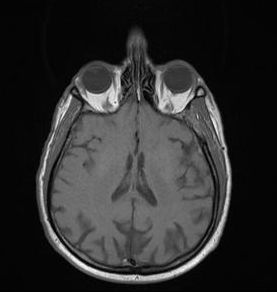
\includegraphics[height=3cm]{images/5009-dkfz-t1}

            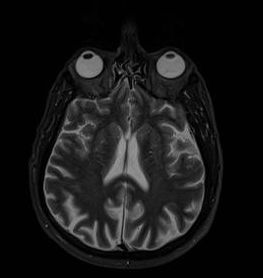
\includegraphics[height=3cm]{images/5009-dkfz-t2}
        \end{figure}
    \end{columns}
\end{frame}

\begin{frame}{Net Magnetization $\rightarrow$ Voxels}

    \begin{columns}
        \column{0.7\linewidth}
        \begin{itemize}
            \item So far, we've looked at the measurable net magnetization of all excited spins
            \item To distinguish between tissue types: overlay the imaging volume with a voxel grid, look at the magnetization within each voxel
            \item Voxel magnetization cannot be measured directly, we'll solve this problem later
        \end{itemize}

        \column{0.3\linewidth}
        \begin{center}
            \begin{tikzpicture}[scale=1.4]
                \only<1>{\node at (0,0.25) [anchor=south west] {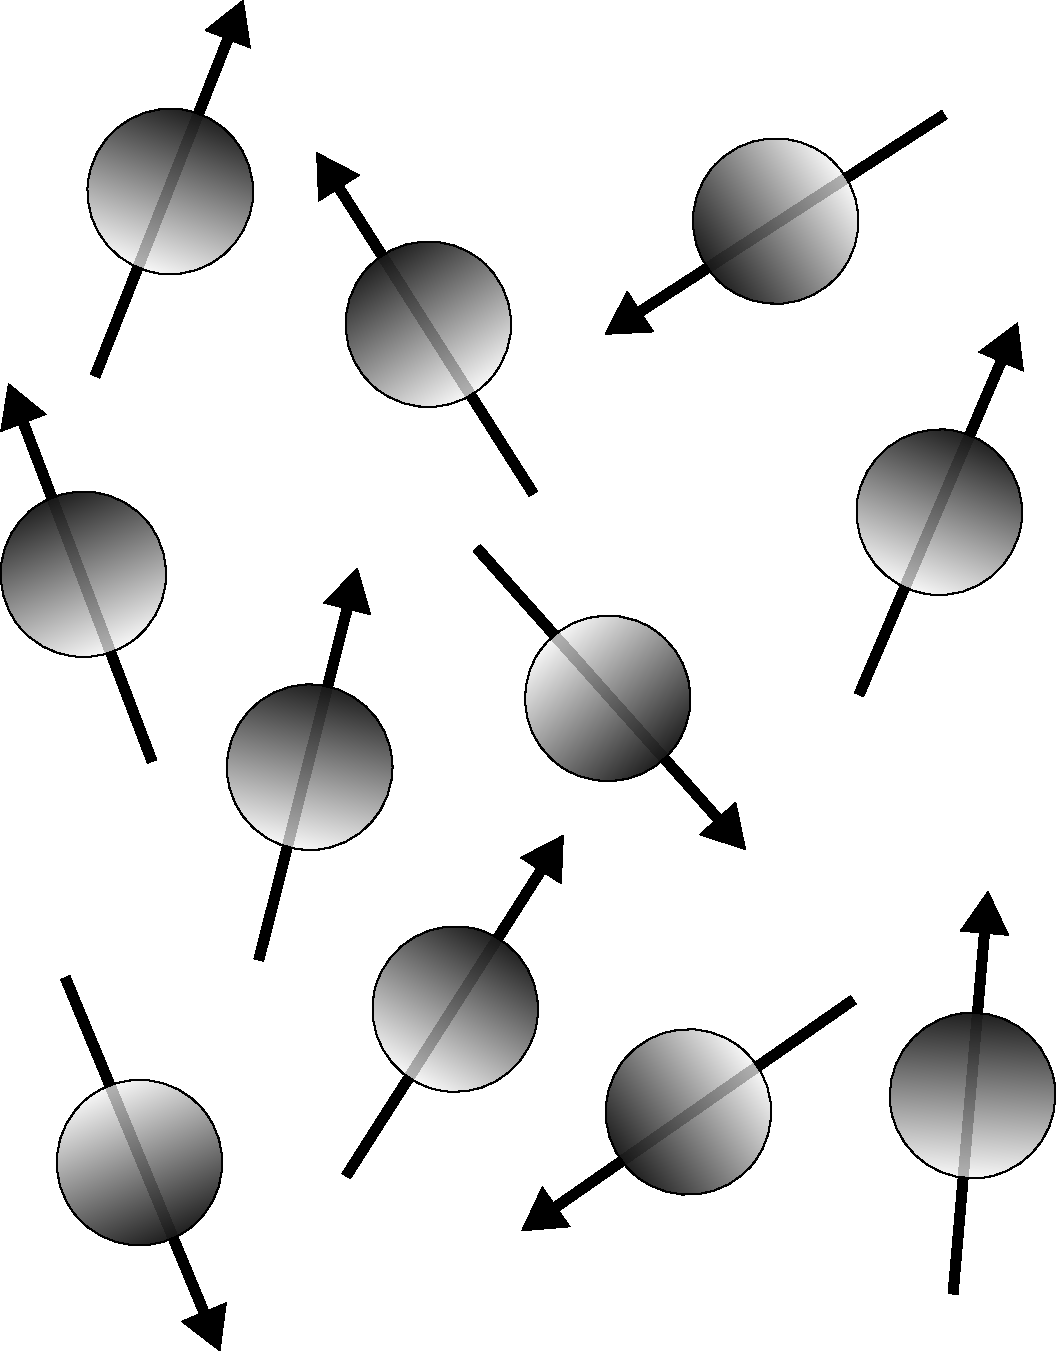
\includegraphics[scale=0.14]{images/random_spins}};}
                \only<2>{
                    \begin{scope}[opacity=0.3]
                        \node at (0,0.25) [anchor=south west] {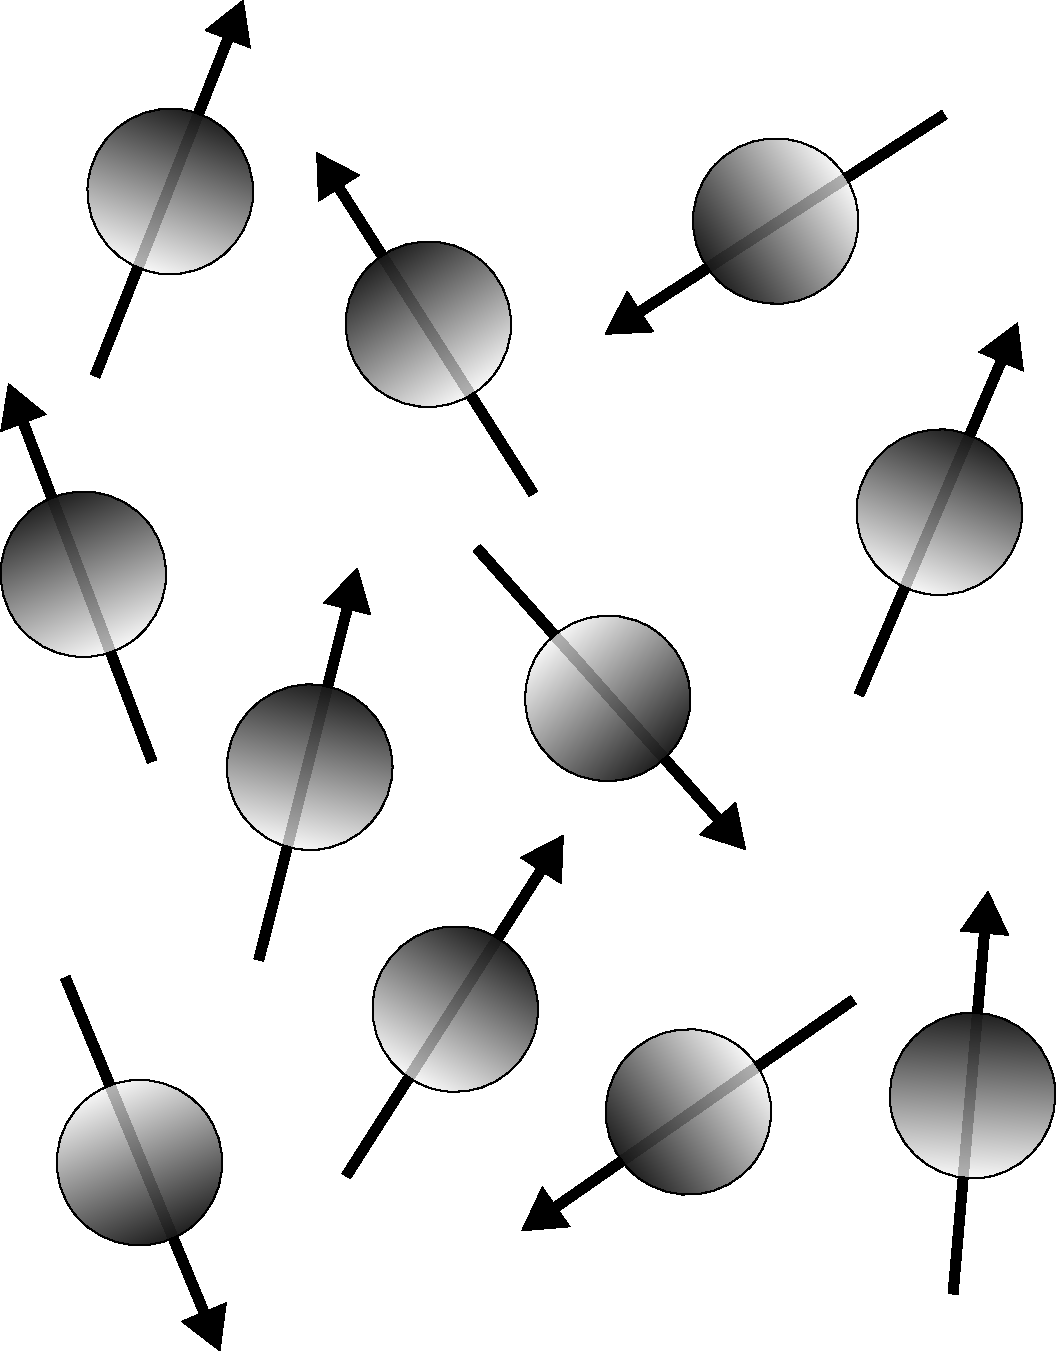
\includegraphics[scale=0.14]{images/random_spins}};
                    \end{scope}}
                \visible<2>{\draw (0, 0) grid (2, 3);
                    \begin{scope}[shift={(0.5,2.5)},rotate=0]
                        \draw[ultra thick,->] (0, -0.25) -- (0, 0.25);
                    \end{scope}
                    \begin{scope}[shift={(1.5,2.5)},rotate=120]
                        \draw[ultra thick,->] (0, -0.25) -- (0, 0.25);
                    \end{scope}
                    \begin{scope}[shift={(0.5,1.5)},rotate=0]
                        \draw[ultra thick,->] (0, -0.23) -- (0, 0.23);
                    \end{scope}
                    \begin{scope}[shift={(1.5,1.5)},rotate=260]
                        \draw[ultra thick,->] (0, -0.1) -- (0, 0.1);
                    \end{scope}
                    \begin{scope}[shift={(0.5,0.5)},rotate=250]
                        \draw[ultra thick,->] (0, -0.12) -- (0, 0.12);
                    \end{scope}
                    \begin{scope}[shift={(1.5,0.5)},rotate=10]
                        \draw[ultra thick,->] (0, -0.1) -- (0, 0.1);
                    \end{scope}
                }
            \end{tikzpicture}
        \end{center}
    \end{columns}

\end{frame}

\begin{frame}{Recap: Excitation}

    \begin{itemize}
        \item Assume \B0 is aligned with the $z$ axis of a coordinate system
        \item Split per-voxel magnetization ${\color{red}\magn{}} = {\color{blue}\magnlong{}} + {\color{green!70!black}\magntrans{}}$ into 2 components:
              \begin{itemize}
                  \item \emph{Longitudinal} component ${\color{blue}\magnlong{}}$ parallel to \B0
                  \item \emph{Transversal}  component ${\color{green!70!black}\magntrans{}}$ orthogonal to \B0
              \end{itemize}
        \item Initially, per-voxel magnetization vectors {\color{red}\magn{}} are aligned with \B0: \\
              $\Vert {\color{green!70!black}\magntrans{}} \Vert = 0$, $\Vert {\color{blue}\magnlong{}} \Vert$ is maximal
        \item After excitation:  $\Vert {\color{blue}\magnlong{}} \Vert = 0$, $\Vert {\color{green!70!black}\magntrans{}} \Vert$ is maximal
    \end{itemize}

    \begin{center}
        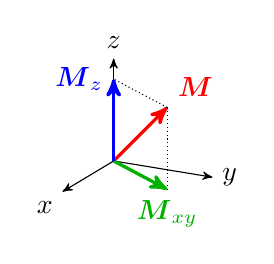
\begin{tikzpicture}[x  = {(-0.5cm,-0.3cm)},
                y  = {(0.9659cm,-0.15882cm)},
                z  = {(0cm,1cm)},
                >=stealth', scale=1.3]
            \draw[->] (0, 0, 0) -- (1, 0, 0) node [below left] {$x$};
            \draw[->] (0, 0, 0) -- (0, 1, 0) node [right] {$y$};
            \draw[->] (0, 0, 0) -- (0, 0, 1) node [above] {$z$};
            \draw[red, very thick, ->] (0, 0, 0) -- (0.5, 0.8, 0.8) node [above right] {$\magn$};
            \draw[green!70!black, very thick, ->] (0, 0, 0) -- (0.5, 0.8, 0) node [below] {$\magntrans$};
            \draw[blue, very thick, ->] (0, 0, 0) -- (0, 0, 0.8) node [left] {$\magnlong$};
            \draw[densely dotted] (0.5, 0.8, 0.8) -- (0.5, 0.8, 0);
            \draw[densely dotted] (0.5, 0.8, 0.8) -- (0, 0, 0.8);
        \end{tikzpicture}
    \end{center}
\end{frame}

\begin{frame}{Relaxation: 2 Processes}

    \begin{itemize}
        \item At this point, two independent processes lead to the realignment of each magnetization vector \magn{} with the main magnetic field \B0:
              \begin{itemize}
                  \item Recovery of the longitudinal component $\Vert \magnlong{} \Vert$
                  \item Decay of the transversal component $\Vert \magntrans{} \Vert$
              \end{itemize}
        \item Happens on different time scales, usually the decay is much faster
    \end{itemize}
\end{frame}

\begin{frame}{Longitudinal Magnetization Recovery}

    \begin{center}
        \tikzsetnextfilename{mr_longitudinal_magnetization_recovery}
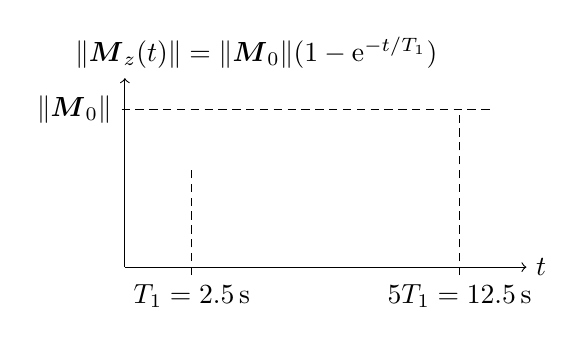
\begin{tikzpicture}[yscale=2,xscale=0.85]
	\draw[->] (0, 0) -- (0, 1.2) node (yl) [above right,xshift=-5ex] {$\Vert\magnlong(t)\Vert=\Vert\magnzero\Vert (1-\mathrm{e}^{-t/\longtime})$};
	\draw[->] (0, 0) -- (6, 0) node [right] {$t$};
	\draw[densely dashed] (1, -0.05) node [below] {$\longtime = 2.5\,\textrm{s}$} -- (1, 0.63);
	\draw[densely dashed] (5, -0.05) node [below] {$5\longtime = 12.5\,\textrm{s}$} -- (5, 0.97);
	\draw[domain=0:5.5,samples=100,very thick] plot[id=mr_t1_recovery] function{1-exp(-x)};
	\draw[densely dashed] (-0.05, 1) node [left] {$\Vert\magnzero{}\Vert$} -- (5.5, 1);
\end{tikzpicture}
    \end{center}

    \begin{itemize}
        \item Exponential recovery of longitudinal magnetization with a time constant \longtime{}, which is tissue-dependent
        \item Reason: spin-lattice relaxation, transfer of received energy into surrounding lattice
    \end{itemize}
\end{frame}

\begin{frame}{Transversal Magnetization Decay (in theory)}

    \begin{center}
        \tikzsetnextfilename{mr_transverse_magnetization_recovery}
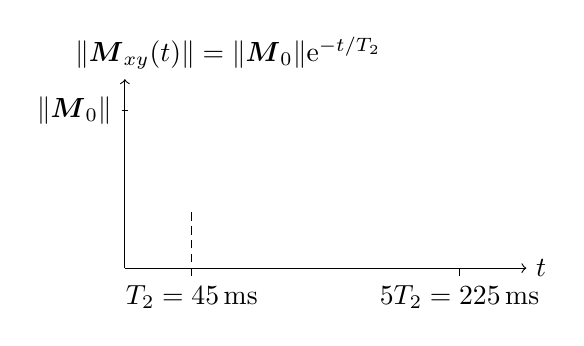
\begin{tikzpicture}[yscale=2,xscale=0.85]
	\draw[->] (0, 0) -- (0, 1.2) node [above right,xshift=-5ex] {$\Vert\magntrans(t)\Vert=\Vert\magnzero\Vert \mathrm{e}^{-t/\transtime}$};
	\draw[->] (0, 0) -- (6, 0) node [right] {$t$};
	\draw[densely dashed] (1, -0.05) node [below] {$\transtime = 45\,\textrm{ms}$} -- (1, 0.37);
	\draw[densely dashed] (5, -0.05) node [below] {$5\transtime = 225\,\textrm{ms}$} -- (5, 0.03);
	\draw[domain=0:5.5,samples=100,very thick] plot[id=mr_t2_recovery] function{exp(-x)};
	\draw[densely dashed] (-0.05, 1) node [left] {$\Vert\magnzero{}\Vert$} -- (0.05, 1);
\end{tikzpicture}
    \end{center}

    \begin{itemize}
        \item Exponential decay of transversal magnetization with a time constant \transtime{}, which is tissue-dependent
        \item Assumes a perfectly homogeneous magnetic field
        \item Reason: interactions of the magnetic fields of nuclei cause dephasing in the $xy$ plane
    \end{itemize}
\end{frame}

\begin{frame}{Transversal Magnetization Decay (in practice)}

    \begin{itemize}
        \item Reality: main magnetic field \B0 is not perfectly homogeneous, due to e.\,g.~magnet manufacture
        \item Inhomogeneity leads to different Larmor frequencies/precession speeds at different spatial locations
        \item $\rightarrow$ Much faster dephasing than according to $\transtime{}$
        \item Time constant $\inhomogtime{}$ (``T two star''), which is always smaller than $\transtime{}$
    \end{itemize}
\end{frame}

\begin{frame}{Combined Relaxation}

    \begin{center}
        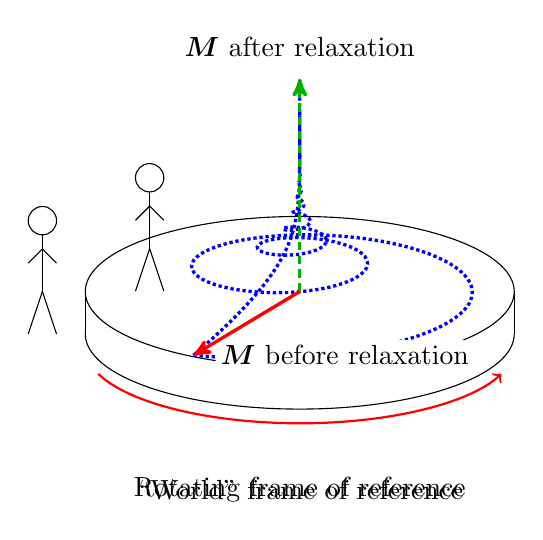
\begin{tikzpicture}[scale=1.8]
            %\draw[draw=none] (-2.5,-1.4) rectangle (2.7,2.5);

            \draw (0, -0.3) ellipse (10ex and 3.5ex);
            \fill[white] (-10ex, 0) -- (10ex, 0) -- (10ex, -0.3) -- (-10ex, -0.3) -- cycle;
            \draw (-10ex, 0) -- (-10ex, -0.3);
            \draw ( 10ex, 0) -- ( 10ex, -0.3);
            \draw[fill=white] (0, 0) ellipse (10ex and 3.5ex);

            \draw[red, thick, ->] (0, -0.4) + (200:10ex and 3.5ex) arc (200:340:10ex and 3.5ex);

            % Stick figure
            \visible<1>{\draw (-12ex, 0.5) circle (0.1);
                \draw (-12ex, 0.4) -- (-12ex, 0);
                \draw (-12ex, 0.3) -- ++(0.1, -0.1);
                \draw (-12ex, 0.3) -- ++(-0.1, -0.1);
                \draw (-12ex, 0) -- ++(0.1, -0.3);
                \draw (-12ex, 0) -- ++(-0.1, -0.3);}

            \visible<1>{\draw (0, -1.4) node {``World'' frame of reference};}
            \visible<2>{\draw (0, -1.4) node {Rotating frame of reference};}

            \visible<2>{
                \begin{scope}[xshift=5ex, yshift=2ex]
                    \draw (-12ex, 0.5) circle (0.1);
                    \draw (-12ex, 0.4) -- (-12ex, 0);
                    \draw (-12ex, 0.3) -- ++(0.1, -0.1);
                    \draw (-12ex, 0.3) -- ++(-0.1, -0.1);
                    \draw (-12ex, 0) -- ++(0.1, -0.3);
                    \draw (-12ex, 0) -- ++(-0.1, -0.3);
                \end{scope}
            }

            \begin{scope}[%overlay,
                    x  = {(-0.5cm,-0.3cm)},
                    y  = {(0.9659cm,-0.15882cm)},
                    z  = {(0cm,1cm)},
                    scale = 1.5,
                    >=stealth']
                %\draw[->] (-1.2, 0, 0) -- (1.2, 0, 0) node [below left] {$x$};
                %\draw[->] (0, -1.2, 0) -- (0, 1.2, 0) node [right] {$y$};
                %\draw[->] (0, 0, -0.2) -- (0, 0, 1) node [above] {$z$};

                \visible<1>{\draw[very thick, blue, densely dotted] ( 1.0000,  0.0000,  0.0000) -- ( 1.0000,  0.0000,  0.0000) -- ( 1.0000,  0.0000,  0.0000) -- ( 1.0000,  0.0000,  0.0000) -- ( 1.0000,  0.0000,  0.0000) -- ( 1.0000,  0.0000,  0.0000) -- ( 1.0000,  0.0000,  0.0000) -- ( 1.0000,  0.0000,  0.0000) -- ( 1.0000,  0.0000,  0.0000) -- ( 1.0000,  0.0000,  0.0000) -- ( 1.0000,  0.0000,  0.0000) -- ( 1.0000,  0.0001,  0.0000) -- ( 1.0000,  0.0001,  0.0000) -- ( 1.0000,  0.0001,  0.0000) -- ( 1.0000,  0.0002,  0.0000) -- ( 1.0000,  0.0002,  0.0000) -- ( 1.0000,  0.0003,  0.0000) -- ( 1.0000,  0.0003,  0.0000) -- ( 0.9999,  0.0004,  0.0000) -- ( 0.9999,  0.0005,  0.0000) -- ( 0.9999,  0.0006,  0.0000) -- ( 0.9999,  0.0008,  0.0000) -- ( 0.9999,  0.0009,  0.0000) -- ( 0.9998,  0.0011,  0.0000) -- ( 0.9998,  0.0013,  0.0000) -- ( 0.9998,  0.0015,  0.0000) -- ( 0.9997,  0.0018,  0.0000) -- ( 0.9997,  0.0021,  0.0000) -- ( 0.9996,  0.0024,  0.0000) -- ( 0.9996,  0.0028,  0.0001) -- ( 0.9995,  0.0032,  0.0001) -- ( 0.9994,  0.0037,  0.0001) -- ( 0.9994,  0.0042,  0.0001) -- ( 0.9993,  0.0047,  0.0001) -- ( 0.9992,  0.0053,  0.0001) -- ( 0.9991,  0.0059,  0.0001) -- ( 0.9990,  0.0067,  0.0001) -- ( 0.9989,  0.0074,  0.0001) -- ( 0.9987,  0.0083,  0.0002) -- ( 0.9986,  0.0092,  0.0002) -- ( 0.9984,  0.0101,  0.0002) -- ( 0.9983,  0.0112,  0.0002) -- ( 0.9981,  0.0123,  0.0002) -- ( 0.9979,  0.0135,  0.0003) -- ( 0.9977,  0.0148,  0.0003) -- ( 0.9975,  0.0162,  0.0003) -- ( 0.9972,  0.0177,  0.0003) -- ( 0.9969,  0.0193,  0.0004) -- ( 0.9967,  0.0210,  0.0004) -- ( 0.9964,  0.0228,  0.0004) -- ( 0.9960,  0.0247,  0.0005) -- ( 0.9957,  0.0267,  0.0005) -- ( 0.9953,  0.0289,  0.0006) -- ( 0.9949,  0.0311,  0.0006) -- ( 0.9944,  0.0336,  0.0007) -- ( 0.9940,  0.0361,  0.0007) -- ( 0.9935,  0.0388,  0.0008) -- ( 0.9929,  0.0416,  0.0008) -- ( 0.9924,  0.0446,  0.0009) -- ( 0.9917,  0.0477,  0.0009) -- ( 0.9911,  0.0510,  0.0010) -- ( 0.9904,  0.0544,  0.0011) -- ( 0.9896,  0.0581,  0.0011) -- ( 0.9888,  0.0619,  0.0012) -- ( 0.9880,  0.0658,  0.0013) -- ( 0.9871,  0.0700,  0.0014) -- ( 0.9861,  0.0744,  0.0015) -- ( 0.9850,  0.0789,  0.0016) -- ( 0.9839,  0.0836,  0.0017) -- ( 0.9828,  0.0886,  0.0018) -- ( 0.9815,  0.0938,  0.0019) -- ( 0.9801,  0.0991,  0.0020) -- ( 0.9787,  0.1047,  0.0021) -- ( 0.9772,  0.1105,  0.0022) -- ( 0.9756,  0.1166,  0.0023) -- ( 0.9738,  0.1229,  0.0024) -- ( 0.9720,  0.1294,  0.0026) -- ( 0.9700,  0.1361,  0.0027) -- ( 0.9679,  0.1431,  0.0029) -- ( 0.9657,  0.1504,  0.0030) -- ( 0.9633,  0.1579,  0.0032) -- ( 0.9608,  0.1657,  0.0033) -- ( 0.9581,  0.1737,  0.0035) -- ( 0.9553,  0.1820,  0.0037) -- ( 0.9522,  0.1905,  0.0038) -- ( 0.9490,  0.1994,  0.0040) -- ( 0.9456,  0.2084,  0.0042) -- ( 0.9420,  0.2178,  0.0044) -- ( 0.9381,  0.2275,  0.0046) -- ( 0.9340,  0.2374,  0.0048) -- ( 0.9297,  0.2476,  0.0051) -- ( 0.9251,  0.2580,  0.0053) -- ( 0.9202,  0.2688,  0.0055) -- ( 0.9151,  0.2798,  0.0058) -- ( 0.9096,  0.2911,  0.0060) -- ( 0.9039,  0.3026,  0.0063) -- ( 0.8977,  0.3144,  0.0065) -- ( 0.8913,  0.3265,  0.0068) -- ( 0.8844,  0.3388,  0.0071) -- ( 0.8772,  0.3514,  0.0074) -- ( 0.8696,  0.3642,  0.0077) -- ( 0.8616,  0.3773,  0.0080) -- ( 0.8531,  0.3906,  0.0083) -- ( 0.8441,  0.4041,  0.0087) -- ( 0.8347,  0.4178,  0.0090) -- ( 0.8248,  0.4316,  0.0094) -- ( 0.8144,  0.4457,  0.0097) -- ( 0.8034,  0.4599,  0.0101) -- ( 0.7918,  0.4743,  0.0105) -- ( 0.7797,  0.4887,  0.0109) -- ( 0.7670,  0.5033,  0.0113) -- ( 0.7536,  0.5180,  0.0117) -- ( 0.7397,  0.5327,  0.0121) -- ( 0.7250,  0.5474,  0.0125) -- ( 0.7097,  0.5621,  0.0130) -- ( 0.6936,  0.5768,  0.0134) -- ( 0.6768,  0.5915,  0.0139) -- ( 0.6593,  0.6060,  0.0144) -- ( 0.6411,  0.6204,  0.0149) -- ( 0.6220,  0.6346,  0.0154) -- ( 0.6022,  0.6486,  0.0159) -- ( 0.5815,  0.6623,  0.0164) -- ( 0.5601,  0.6758,  0.0170) -- ( 0.5378,  0.6888,  0.0176) -- ( 0.5147,  0.7015,  0.0181) -- ( 0.4908,  0.7136,  0.0187) -- ( 0.4660,  0.7253,  0.0193) -- ( 0.4403,  0.7364,  0.0199) -- ( 0.4138,  0.7468,  0.0206) -- ( 0.3865,  0.7565,  0.0212) -- ( 0.3584,  0.7654,  0.0219) -- ( 0.3295,  0.7735,  0.0225) -- ( 0.2997,  0.7807,  0.0232) -- ( 0.2693,  0.7869,  0.0239) -- ( 0.2380,  0.7921,  0.0246) -- ( 0.2061,  0.7961,  0.0254) -- ( 0.1735,  0.7989,  0.0261) -- ( 0.1403,  0.8005,  0.0269) -- ( 0.1065,  0.8006,  0.0277) -- ( 0.0722,  0.7994,  0.0285) -- ( 0.0375,  0.7967,  0.0293) -- ( 0.0024,  0.7923,  0.0301) -- (-0.0330,  0.7864,  0.0310) -- (-0.0686,  0.7787,  0.0318) -- (-0.1043,  0.7693,  0.0327) -- (-0.1400,  0.7580,  0.0336) -- (-0.1756,  0.7448,  0.0345) -- (-0.2109,  0.7297,  0.0355) -- (-0.2459,  0.7126,  0.0364) -- (-0.2804,  0.6935,  0.0374) -- (-0.3143,  0.6724,  0.0384) -- (-0.3474,  0.6492,  0.0394) -- (-0.3795,  0.6239,  0.0405) -- (-0.4106,  0.5966,  0.0415) -- (-0.4403,  0.5672,  0.0426) -- (-0.4687,  0.5358,  0.0437) -- (-0.4954,  0.5024,  0.0448) -- (-0.5203,  0.4671,  0.0459) -- (-0.5432,  0.4300,  0.0471) -- (-0.5639,  0.3912,  0.0482) -- (-0.5823,  0.3507,  0.0494) -- (-0.5982,  0.3088,  0.0507) -- (-0.6114,  0.2655,  0.0519) -- (-0.6218,  0.2210,  0.0531) -- (-0.6291,  0.1756,  0.0544) -- (-0.6332,  0.1294,  0.0557) -- (-0.6341,  0.0827,  0.0571) -- (-0.6315,  0.0357,  0.0584) -- (-0.6255, -0.0113,  0.0598) -- (-0.6158, -0.0581,  0.0612) -- (-0.6025, -0.1042,  0.0626) -- (-0.5856, -0.1495,  0.0640) -- (-0.5650, -0.1935,  0.0655) -- (-0.5408, -0.2360,  0.0670) -- (-0.5131, -0.2765,  0.0685) -- (-0.4819, -0.3148,  0.0700) -- (-0.4475, -0.3504,  0.0715) -- (-0.4099, -0.3831,  0.0731) -- (-0.3694, -0.4124,  0.0747) -- (-0.3264, -0.4381,  0.0764) -- (-0.2810, -0.4599,  0.0780) -- (-0.2337, -0.4774,  0.0797) -- (-0.1848, -0.4904,  0.0814) -- (-0.1348, -0.4987,  0.0831) -- (-0.0841, -0.5022,  0.0849) -- (-0.0332, -0.5006,  0.0866) -- ( 0.0173, -0.4939,  0.0884) -- ( 0.0669, -0.4821,  0.0903) -- ( 0.1151, -0.4652,  0.0921) -- ( 0.1612, -0.4433,  0.0940) -- ( 0.2047, -0.4166,  0.0959) -- ( 0.2451, -0.3854,  0.0978) -- ( 0.2817, -0.3499,  0.0998) -- ( 0.3141, -0.3106,  0.1018) -- ( 0.3418, -0.2679,  0.1038) -- ( 0.3643, -0.2224,  0.1058) -- ( 0.3813, -0.1746,  0.1079) -- ( 0.3924, -0.1253,  0.1100) -- ( 0.3975, -0.0751,  0.1121) -- ( 0.3963, -0.0249,  0.1143) -- ( 0.3890,  0.0246,  0.1164) -- ( 0.3755,  0.0726,  0.1186) -- ( 0.3560,  0.1183,  0.1209) -- ( 0.3308,  0.1609,  0.1231) -- ( 0.3004,  0.1996,  0.1254) -- ( 0.2652,  0.2336,  0.1277) -- ( 0.2260,  0.2624,  0.1300) -- ( 0.1834,  0.2853,  0.1324) -- ( 0.1383,  0.3019,  0.1348) -- ( 0.0916,  0.3119,  0.1372) -- ( 0.0444,  0.3150,  0.1397) -- (-0.0025,  0.3112,  0.1422) -- (-0.0480,  0.3006,  0.1447) -- (-0.0909,  0.2833,  0.1472) -- (-0.1304,  0.2600,  0.1498) -- (-0.1654,  0.2310,  0.1524) -- (-0.1952,  0.1972,  0.1550) -- (-0.2190,  0.1595,  0.1576) -- (-0.2362,  0.1189,  0.1603) -- (-0.2465,  0.0765,  0.1630) -- (-0.2495,  0.0334,  0.1658) -- (-0.2453, -0.0091,  0.1685) -- (-0.2340, -0.0498,  0.1713) -- (-0.2161, -0.0874,  0.1741) -- (-0.1922, -0.1209,  0.1770) -- (-0.1631, -0.1492,  0.1799) -- (-0.1299, -0.1716,  0.1828) -- (-0.0936, -0.1873,  0.1857) -- (-0.0556, -0.1959,  0.1887) -- (-0.0173, -0.1972,  0.1916) -- ( 0.0200, -0.1914,  0.1947) -- ( 0.0550, -0.1787,  0.1977) -- ( 0.0863, -0.1597,  0.2008) -- ( 0.1129, -0.1354,  0.2039) -- ( 0.1337, -0.1068,  0.2070) -- ( 0.1480, -0.0751,  0.2102) -- ( 0.1554, -0.0417,  0.2134) -- ( 0.1558, -0.0081,  0.2166) -- ( 0.1492,  0.0241,  0.2198) -- ( 0.1362,  0.0537,  0.2231) -- ( 0.1175,  0.0793,  0.2264) -- ( 0.0942,  0.0997,  0.2297) -- ( 0.0674,  0.1143,  0.2331) -- ( 0.0388,  0.1223,  0.2364) -- ( 0.0096,  0.1236,  0.2398) -- (-0.0184,  0.1184,  0.2433) -- (-0.0439,  0.1071,  0.2467) -- (-0.0655,  0.0905,  0.2502) -- (-0.0822,  0.0697,  0.2537) -- (-0.0931,  0.0462,  0.2573) -- (-0.0979,  0.0213,  0.2608) -- (-0.0965, -0.0034,  0.2644) -- (-0.0892, -0.0264,  0.2680) -- (-0.0767, -0.0463,  0.2716) -- (-0.0599, -0.0619,  0.2753) -- (-0.0403, -0.0725,  0.2790) -- (-0.0192, -0.0774,  0.2827) -- ( 0.0019, -0.0766,  0.2864) -- ( 0.0215, -0.0704,  0.2902) -- ( 0.0381, -0.0595,  0.2940) -- ( 0.0508, -0.0449,  0.2978) -- ( 0.0588, -0.0279,  0.3016) -- ( 0.0616, -0.0099,  0.3055) -- ( 0.0593,  0.0076,  0.3094) -- ( 0.0523,  0.0232,  0.3133) -- ( 0.0415,  0.0358,  0.3172) -- ( 0.0280,  0.0444,  0.3211) -- ( 0.0130,  0.0484,  0.3251) -- (-0.0020,  0.0479,  0.3291) -- (-0.0156,  0.0430,  0.3331) -- (-0.0268,  0.0346,  0.3371) -- (-0.0345,  0.0235,  0.3412) -- (-0.0383,  0.0110,  0.3452) -- (-0.0379, -0.0016,  0.3493) -- (-0.0338, -0.0129,  0.3534) -- (-0.0265, -0.0220,  0.3575) -- (-0.0170, -0.0280,  0.3617) -- (-0.0065, -0.0305,  0.3658) -- ( 0.0038, -0.0294,  0.3700) -- ( 0.0128, -0.0251,  0.3742) -- ( 0.0196, -0.0183,  0.3784) -- ( 0.0234, -0.0100,  0.3827) -- ( 0.0241, -0.0012,  0.3869) -- ( 0.0218,  0.0070,  0.3912) -- ( 0.0170,  0.0135,  0.3955) -- ( 0.0105,  0.0177,  0.3997) -- ( 0.0032,  0.0192,  0.4041) -- (-0.0038,  0.0180,  0.4084) -- (-0.0096,  0.0145,  0.4127) -- (-0.0135,  0.0094,  0.4171) -- (-0.0152,  0.0034,  0.4214) -- (-0.0144, -0.0025,  0.4258) -- (-0.0117, -0.0074,  0.4302) -- (-0.0075, -0.0107,  0.4346) -- (-0.0026, -0.0120,  0.4390) -- ( 0.0022, -0.0113,  0.4434) -- ( 0.0062, -0.0090,  0.4478) -- ( 0.0087, -0.0054,  0.4523) -- ( 0.0095, -0.0013,  0.4567) -- ( 0.0087,  0.0026,  0.4612) -- ( 0.0064,  0.0055,  0.4656) -- ( 0.0033,  0.0072,  0.4701) -- (-0.0001,  0.0075,  0.4746) -- (-0.0030,  0.0063,  0.4790) -- (-0.0051,  0.0041,  0.4835) -- (-0.0060,  0.0014,  0.4880) -- (-0.0056, -0.0012,  0.4925) -- (-0.0042, -0.0033,  0.4970) -- (-0.0021, -0.0045,  0.5015) -- ( 0.0002, -0.0047,  0.5060) -- ( 0.0021, -0.0038,  0.5105) -- ( 0.0034, -0.0023,  0.5151) -- ( 0.0037, -0.0004,  0.5196) -- ( 0.0033,  0.0013,  0.5241) -- ( 0.0021,  0.0025,  0.5286) -- ( 0.0007,  0.0030,  0.5331) -- (-0.0008,  0.0027,  0.5376) -- (-0.0018,  0.0019,  0.5422) -- (-0.0023,  0.0007,  0.5467) -- (-0.0022, -0.0005,  0.5512) -- (-0.0015, -0.0014,  0.5557) -- (-0.0006, -0.0018,  0.5602) -- ( 0.0004, -0.0017,  0.5647) -- ( 0.0011, -0.0012,  0.5692) -- ( 0.0015, -0.0004,  0.5737) -- ( 0.0014,  0.0004,  0.5782) -- ( 0.0009,  0.0009,  0.5826) -- ( 0.0002,  0.0012,  0.5871) -- (-0.0004,  0.0010,  0.5916) -- (-0.0008,  0.0006,  0.5960) -- (-0.0009,  0.0001,  0.6005) -- (-0.0008, -0.0004,  0.6049) -- (-0.0004, -0.0007,  0.6093) -- ( 0.0001, -0.0007,  0.6138) -- ( 0.0004, -0.0005,  0.6182) -- ( 0.0006, -0.0002,  0.6226) -- ( 0.0005,  0.0002,  0.6269) -- ( 0.0003,  0.0004,  0.6313) -- ( 0.0000,  0.0005,  0.6357) -- (-0.0002,  0.0004,  0.6400) -- (-0.0004,  0.0001,  0.6444) -- (-0.0003, -0.0001,  0.6487) -- (-0.0002, -0.0002,  0.6530) -- (-0.0000, -0.0003,  0.6573) -- ( 0.0001, -0.0002,  0.6615) -- ( 0.0002, -0.0001,  0.6658) -- ( 0.0002,  0.0001,  0.6700) -- ( 0.0001,  0.0002,  0.6743) -- (-0.0000,  0.0002,  0.6785) -- (-0.0001,  0.0001,  0.6826) -- (-0.0001,  0.0000,  0.6868) -- (-0.0001, -0.0001,  0.6910) -- (-0.0000, -0.0001,  0.6951) -- ( 0.0000, -0.0001,  0.6992) -- ( 0.0001, -0.0000,  0.7033) -- ( 0.0001,  0.0000,  0.7073) -- ( 0.0000,  0.0001,  0.7114) -- (-0.0000,  0.0001,  0.7154) -- (-0.0000,  0.0000,  0.7194) -- (-0.0001,  0.0000,  0.7234) -- (-0.0000, -0.0000,  0.7273) -- (-0.0000, -0.0000,  0.7312) -- ( 0.0000, -0.0000,  0.7351) -- ( 0.0000, -0.0000,  0.7390) -- ( 0.0000,  0.0000,  0.7429) -- ( 0.0000,  0.0000,  0.7467) -- (-0.0000,  0.0000,  0.7505) -- (-0.0000,  0.0000,  0.7543) -- (-0.0000, -0.0000,  0.7580) -- (-0.0000, -0.0000,  0.7617) -- ( 0.0000, -0.0000,  0.7654) -- ( 0.0000, -0.0000,  0.7691) -- ( 0.0000,  0.0000,  0.7727) -- ( 0.0000,  0.0000,  0.7763) -- (-0.0000,  0.0000,  0.7799) -- (-0.0000,  0.0000,  0.7834) -- (-0.0000, -0.0000,  0.7870) -- ( 0.0000, -0.0000,  0.7905) -- ( 0.0000, -0.0000,  0.7939) -- ( 0.0000,  0.0000,  0.7973) -- ( 0.0000,  0.0000,  0.8007) -- (-0.0000,  0.0000,  0.8041) -- (-0.0000,  0.0000,  0.8074) -- (-0.0000, -0.0000,  0.8108) -- (-0.0000, -0.0000,  0.8140) -- ( 0.0000, -0.0000,  0.8173) -- ( 0.0000,  0.0000,  0.8205) -- ( 0.0000,  0.0000,  0.8237) -- (-0.0000,  0.0000,  0.8268) -- (-0.0000,  0.0000,  0.8299) -- (-0.0000, -0.0000,  0.8330) -- ( 0.0000, -0.0000,  0.8361) -- ( 0.0000, -0.0000,  0.8391) -- ( 0.0000,  0.0000,  0.8420) -- ( 0.0000,  0.0000,  0.8450) -- (-0.0000,  0.0000,  0.8479) -- (-0.0000, -0.0000,  0.8508) -- (-0.0000, -0.0000,  0.8537) -- ( 0.0000, -0.0000,  0.8565) -- ( 0.0000, -0.0000,  0.8593);}

                \visible<2>{\draw[very thick, blue, densely dotted] ( 1.0000, 0,  0.0000)
                    -- ( 0.9281, 0,  0.0098)
                    -- ( 0.8614, 0,  0.0194)
                    -- ( 0.7994, 0,  0.0290)
                    -- ( 0.7419, 0,  0.0385)
                    -- ( 0.6886, 0,  0.0478)
                    -- ( 0.6391, 0,  0.0571)
                    -- ( 0.5931, 0,  0.0663)
                    -- ( 0.5505, 0,  0.0754)
                    -- ( 0.5109, 0,  0.0845)
                    -- ( 0.4741, 0,  0.0934)
                    -- ( 0.4400, 0,  0.1022)
                    -- ( 0.4084, 0,  0.1110)
                    -- ( 0.3790, 0,  0.1197)
                    -- ( 0.3518, 0,  0.1283)
                    -- ( 0.3265, 0,  0.1368)
                    -- ( 0.3030, 0,  0.1452)
                    -- ( 0.2812, 0,  0.1535)
                    -- ( 0.2610, 0,  0.1618)
                    -- ( 0.2422, 0,  0.1700)
                    -- ( 0.2248, 0,  0.1781)
                    -- ( 0.2086, 0,  0.1861)
                    -- ( 0.1936, 0,  0.1940)
                    -- ( 0.1797, 0,  0.2019)
                    -- ( 0.1668, 0,  0.2097)
                    -- ( 0.1548, 0,  0.2174)
                    -- ( 0.1437, 0,  0.2250)
                    -- ( 0.1333, 0,  0.2326)
                    -- ( 0.1237, 0,  0.2401)
                    -- ( 0.1148, 0,  0.2475)
                    -- ( 0.1066, 0,  0.2548)
                    -- ( 0.0989, 0,  0.2621)
                    -- ( 0.0918, 0,  0.2693)
                    -- ( 0.0852, 0,  0.2764)
                    -- ( 0.0791, 0,  0.2835)
                    -- ( 0.0734, 0,  0.2905)
                    -- ( 0.0681, 0,  0.2974)
                    -- ( 0.0632, 0,  0.3042)
                    -- ( 0.0587, 0,  0.3110)
                    -- ( 0.0545, 0,  0.3177)
                    -- ( 0.0505, 0,  0.3244)
                    -- ( 0.0469, 0,  0.3310)
                    -- ( 0.0435, 0,  0.3375)
                    -- ( 0.0404, 0,  0.3440)
                    -- ( 0.0375, 0,  0.3504)
                    -- ( 0.0348, 0,  0.3567)
                    -- ( 0.0323, 0,  0.3630)
                    -- ( 0.0300, 0,  0.3692)
                    -- ( 0.0278, 0,  0.3754)
                    -- ( 0.0258, 0,  0.3815)
                    -- ( 0.0240, 0,  0.3875)
                    -- ( 0.0222, 0,  0.3935)
                    -- ( 0.0206, 0,  0.3994)
                    -- ( 0.0192, 0,  0.4052)
                    -- ( 0.0178, 0,  0.4110)
                    -- ( 0.0165, 0,  0.4168)
                    -- ( 0.0153, 0,  0.4225)
                    -- ( 0.0142, 0,  0.4281)
                    -- ( 0.0132, 0,  0.4337)
                    -- ( 0.0122, 0,  0.4392)
                    -- ( 0.0114, 0,  0.4447)
                    -- ( 0.0105, 0,  0.4501)
                    -- ( 0.0098, 0,  0.4555)
                    -- ( 0.0091, 0,  0.4608)
                    -- ( 0.0084, 0,  0.4660)
                    -- ( 0.0078, 0,  0.4713)
                    -- ( 0.0073, 0,  0.4764)
                    -- ( 0.0067, 0,  0.4815)
                    -- ( 0.0063, 0,  0.4866)
                    -- ( 0.0058, 0,  0.4916)
                    -- ( 0.0054, 0,  0.4966)
                    -- ( 0.0050, 0,  0.5015)
                    -- ( 0.0046, 0,  0.5063)
                    -- ( 0.0043, 0,  0.5111)
                    -- ( 0.0040, 0,  0.5159)
                    -- ( 0.0037, 0,  0.5206)
                    -- ( 0.0034, 0,  0.5253)
                    -- ( 0.0032, 0,  0.5299)
                    -- ( 0.0030, 0,  0.5345)
                    -- ( 0.0028, 0,  0.5391)
                    -- ( 0.0026, 0,  0.5436)
                    -- ( 0.0024, 0,  0.5480)
                    -- ( 0.0022, 0,  0.5524)
                    -- ( 0.0020, 0,  0.5568)
                    -- ( 0.0019, 0,  0.5611)
                    -- ( 0.0018, 0,  0.5654)
                    -- ( 0.0016, 0,  0.5696)
                    -- ( 0.0015, 0,  0.5738)
                    -- ( 0.0014, 0,  0.5780)
                    -- ( 0.0013, 0,  0.5821)
                    -- ( 0.0012, 0,  0.5862)
                    -- ( 0.0011, 0,  0.5902)
                    -- ( 0.0010, 0,  0.5942)
                    -- ( 0.0010, 0,  0.5982)
                    -- ( 0.0009, 0,  0.6021)
                    -- ( 0.0008, 0,  0.6060)
                    -- ( 0.0008, 0,  0.6098)
                    -- ( 0.0007, 0,  0.6136)
                    -- ( 0.0007, 0,  0.6174)
                    -- ( 0.0006, 0,  0.6211)
                    -- ( 0.0006, 0,  0.6248)
                    -- ( 0.0005, 0,  0.6285)
                    -- ( 0.0005, 0,  0.6321)
                    -- ( 0.0005, 0,  0.6357)
                    -- ( 0.0004, 0,  0.6393)
                    -- ( 0.0004, 0,  0.6428)
                    -- ( 0.0004, 0,  0.6463)
                    -- ( 0.0003, 0,  0.6497)
                    -- ( 0.0003, 0,  0.6531)
                    -- ( 0.0003, 0,  0.6565)
                    -- ( 0.0003, 0,  0.6599)
                    -- ( 0.0003, 0,  0.6632)
                    -- ( 0.0002, 0,  0.6665)
                    -- ( 0.0002, 0,  0.6697)
                    -- ( 0.0002, 0,  0.6730)
                    -- ( 0.0002, 0,  0.6761)
                    -- ( 0.0002, 0,  0.6793)
                    -- ( 0.0002, 0,  0.6824)
                    -- ( 0.0001, 0,  0.6855)
                    -- ( 0.0001, 0,  0.6886)
                    -- ( 0.0001, 0,  0.6916)
                    -- ( 0.0001, 0,  0.6946)
                    -- ( 0.0001, 0,  0.6976)
                    -- ( 0.0001, 0,  0.7006)
                    -- ( 0.0001, 0,  0.7035)
                    -- ( 0.0001, 0,  0.7064)
                    -- ( 0.0001, 0,  0.7093)
                    -- ( 0.0001, 0,  0.7121)
                    -- ( 0.0001, 0,  0.7149)
                    -- ( 0.0001, 0,  0.7177)
                    -- ( 0.0001, 0,  0.7204)
                    -- ( 0.0001, 0,  0.7232)
                    -- ( 0.0001, 0,  0.7259)
                    -- ( 0.0000, 0,  0.7285)
                    -- ( 0.0000, 0,  0.9972);}

                \draw[green!70!black,very thick,densely dashed,->] (0, 0, 0) -- (0, 0, 1) node [black,above=1ex] {\magn{} after relaxation};
                \draw[red,very thick,->] (0, 0, 0) -- (1, 0, 0) node [black,right=1.7ex, inner sep=2pt, rounded corners, fill=white] {\magn{} before relaxation};
            \end{scope}
        \end{tikzpicture}
    \end{center}
\end{frame}

\begin{frame}{Image Contrast}

    \begin{itemize}
        \item Two parameters of an image acquisition influence the contrast:
              \begin{itemize}
                  \item \textbf{Echo time (TE):} The time between excitation and the measurement of a magnetization vector
                  \item \textbf{Repetition time (TR):} The time between excitations for the measurement of different magnetization vectors
              \end{itemize}
    \end{itemize}

    \begin{center}
        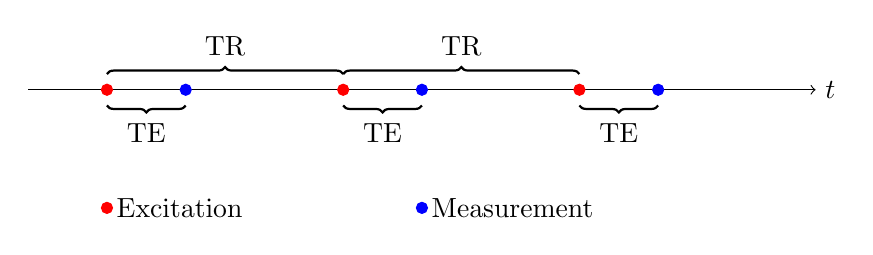
\begin{tikzpicture}
            \draw[->] (0, 0) -- (10, 0) node [right] {$t$};
            \filldraw[red] (1, 0) circle (2pt);
            \filldraw[blue] (2, 0) circle (2pt);
            \filldraw[red] (4, 0) circle (2pt);
            \filldraw[blue] (5, 0) circle (2pt);
            \filldraw[red] (7, 0) circle (2pt);
            \filldraw[blue] (8, 0) circle (2pt);
            \draw [
                thick,
                decoration={
                        brace,
                        mirror,
                        raise=0.2cm
                    },
                decorate
            ] (1, 0) -- node [below=0.3cm] {TE} (2, 0);
            \draw [
                thick,
                decoration={
                        brace,
                        mirror,
                        raise=0.2cm
                    },
                decorate
            ] (4, 0) -- node [below=0.3cm] {TE} (5, 0);
            \draw [
                thick,
                decoration={
                        brace,
                        mirror,
                        raise=0.2cm
                    },
                decorate
            ] (7, 0) -- node [below=0.3cm] {TE} (8, 0);
            \draw [
                thick,
                decoration={
                        brace,
                        raise=0.2cm
                    },
                decorate
            ] (1, 0) -- node [above=0.3cm] {TR} (4, 0);
            \draw [
                thick,
                decoration={
                        brace,
                        raise=0.2cm
                    },
                decorate
            ] (4, 0) -- node [above=0.3cm] {TR} (7, 0);
            \filldraw[red] (1, -1.5) circle (2pt) node [right, black] {Excitation};
            \filldraw[blue] (5, -1.5) circle (2pt) node [right, black] {Measurement};
        \end{tikzpicture}
    \end{center}
\end{frame}

\begin{frame}{\longtime{} Weighting}

    \begin{columns}[t,onlytextwidth]
        \column{.7\linewidth}
        \tikzsetnextfilename{mr_longitudinal_magnetization_recovery_2tissues}
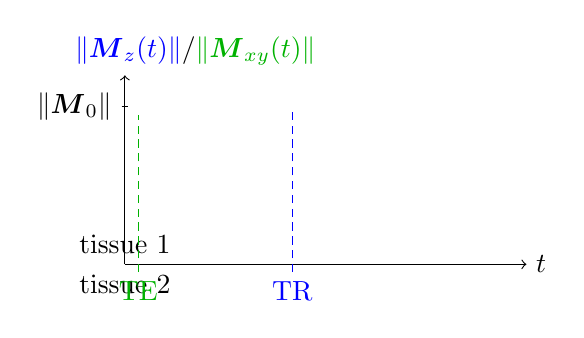
\begin{tikzpicture}[yscale=2,xscale=0.85]
	\draw[->] (0, 0) -- (0, 1.2) node [above right,xshift=-5ex] {{\color{blue}$\Vert\magnlong(t)\Vert$}/{\color{green!70!black}$\Vert\magntrans(t)\Vert$}};
	\draw[->] (0, 0) -- (6, 0) node [right] {$t$};
	% \draw[densely dashed] (1, -0.05) node [below] {$\transtime = 45\,\textrm{ms}$} -- (1, 0.37);
	% \draw[densely dashed] (5, -0.05) node [below] {$5\transtime = 225\,\textrm{ms}$} -- (5, 0.03);
	\draw[domain=0:5.5,samples=100,very thick, green!70!black] plot[id=mr_t2_recovery_tissue1] function{exp(-x/1.5)};
	\draw[domain=0:5.5,samples=100,very thick, green!70!black,densely dotted] plot[id=mr_t2_recovery_tissue2] function{exp(-x/3.5)};
	\draw[domain=0:5.5,samples=100,very thick, blue] plot[id=mr_t1_recovery_tissue1] function{1-exp(-x/0.45)} node [above, black] {tissue 1};
	\draw[domain=0:5.5,samples=100,very thick, blue, densely dotted] plot[id=mr_t1_recovery_tissue2] function{1-exp(-x/2)} node [below, black] {tissue 2};
	\draw[densely dashed] (-0.05, 1) node [left] {$\Vert\magnzero{}\Vert$} -- (0.05, 1);
	\draw[densely dashed,green!70!black] (0.2, -0.05) node [below] {TE} -- (0.2, 0.95);
	\draw[densely dashed,blue] (2.5, -0.05) node [below] {TR} -- (2.5, 1);
\end{tikzpicture}

        \begin{itemize}
            \item \textbf{Short TR:} Not all tissues fully recover magnetization before new measurements
            \item \textbf{Short TE:} Don't allow differences in transversal decay to influence contrast
        \end{itemize}

        \column{.3\linewidth}
        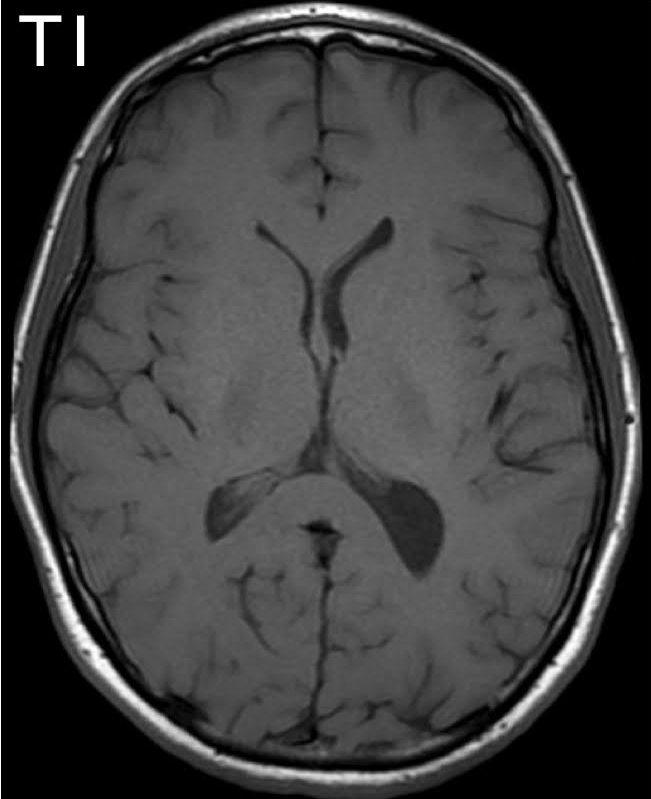
\includegraphics[height=0.6\textheight]{images/t1}

        {\scriptsize Image source: UCSF Dept. of Radiology and Biomedical Imaging}
    \end{columns}
\end{frame}

\begin{frame}{\transtime{} Weighting}

    \begin{columns}[t,onlytextwidth]
        \column{.7\linewidth}
        \tikzsetnextfilename{mr_transverse_magnetization_recovery_2tissues}
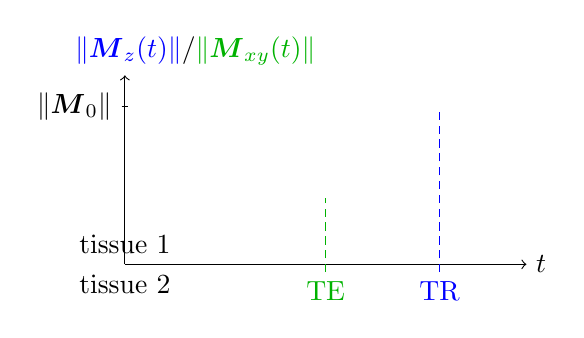
\begin{tikzpicture}[yscale=2,xscale=0.85]
	\draw[->] (0, 0) -- (0, 1.2) node [above right,xshift=-5ex] {{\color{blue}$\Vert\magnlong(t)\Vert$}/{\color{green!70!black}$\Vert\magntrans(t)\Vert$}};
	\draw[->] (0, 0) -- (6, 0) node [right] {$t$};
	% \draw[densely dashed] (1, -0.05) node [below] {$\transtime = 45\,\textrm{ms}$} -- (1, 0.37);
	% \draw[densely dashed] (5, -0.05) node [below] {$5\transtime = 225\,\textrm{ms}$} -- (5, 0.03);
	\draw[domain=0:5.5,samples=100,very thick, green!70!black] plot[id=mr_t2_recovery_tissue1] function{exp(-x/1.5)};
	\draw[domain=0:5.5,samples=100,very thick, green!70!black,densely dotted] plot[id=mr_t2_recovery_tissue2] function{exp(-x/3.5)};
	\draw[domain=0:5.5,samples=100,very thick, blue] plot[id=mr_t1_recovery_tissue1] function{1-exp(-x/0.45)} node [above, black] {tissue 1};
	\draw[domain=0:5.5,samples=100,very thick, blue, densely dotted] plot[id=mr_t1_recovery_tissue2] function{1-exp(-x/2)} node [below, black] {tissue 2};
	\draw[densely dashed] (-0.05, 1) node [left] {$\Vert\magnzero{}\Vert$} -- (0.05, 1);
	\draw[densely dashed,green!70!black] (3, -0.05) node [below] {TE} -- (3, 0.424);
	\draw[densely dashed,blue] (4.7, -0.05) node [below] {TR} -- (4.7, 1);
\end{tikzpicture}

        \begin{itemize}
            \item \textbf{Long TE:} Allow differences in transversal magnetization decay to manifest
            \item \textbf{Long TR:} Longitudinal recovery between measurements to prevent \longtime{} influence
        \end{itemize}

        \column{.3\linewidth}
        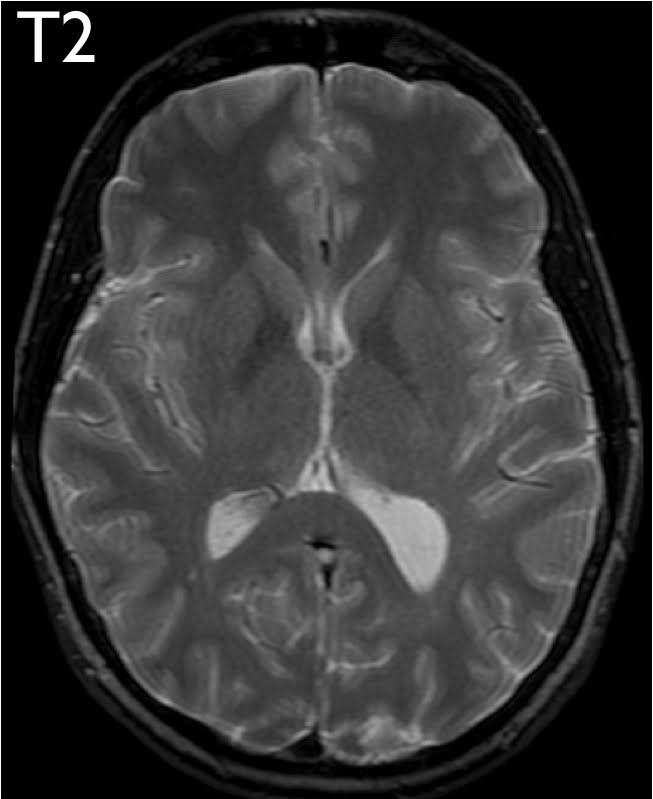
\includegraphics[height=0.6\textheight]{images/t2}

        {\scriptsize Image source: UCSF Dept. of Radiology and Biomedical Imaging}
    \end{columns}
\end{frame}

\begin{frame}{Proton Density (PD) Weighting}

    \begin{columns}[t,onlytextwidth]
        \column{.7\linewidth}
        \tikzsetnextfilename{mr_transverse_magnetization_recovery_2tissues}
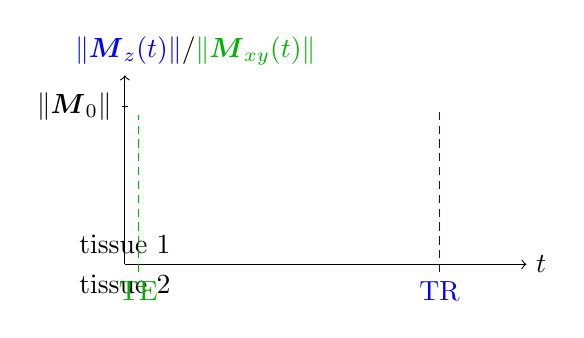
\begin{tikzpicture}[yscale=2,xscale=0.85]
	\draw[->] (0, 0) -- (0, 1.2) node [above right,xshift=-5ex] {{\color{blue}$\Vert\magnlong(t)\Vert$}/{\color{green!70!black}$\Vert\magntrans(t)\Vert$}};
	\draw[->] (0, 0) -- (6, 0) node [right] {$t$};
	% \draw[densely dashed] (1, -0.05) node [below] {$\transtime = 45\,\textrm{ms}$} -- (1, 0.37);
	% \draw[densely dashed] (5, -0.05) node [below] {$5\transtime = 225\,\textrm{ms}$} -- (5, 0.03);
	\draw[domain=0:5.5,samples=100,very thick, green!70!black] plot[id=mr_t2_recovery_tissue1] function{exp(-x/1.5)};
	\draw[domain=0:5.5,samples=100,very thick, green!70!black,densely dotted] plot[id=mr_t2_recovery_tissue2] function{exp(-x/3.5)};
	\draw[domain=0:5.5,samples=100,very thick, blue] plot[id=mr_t1_recovery_tissue1] function{1-exp(-x/0.45)} node [above, black] {tissue 1};
	\draw[domain=0:5.5,samples=100,very thick, blue, densely dotted] plot[id=mr_t1_recovery_tissue2] function{1-exp(-x/2)} node [below, black] {tissue 2};
	\draw[densely dashed] (-0.05, 1) node [left] {$\Vert\magnzero{}\Vert$} -- (0.05, 1);
	\draw[densely dashed,green!70!black] (0.2, -0.05) node [below] {TE} -- (0.2, 0.95);
	\draw[densely dashed,blue] (4.7, -0.05) node [below] {TR} -- (4.7, 1);
\end{tikzpicture}

        \begin{itemize}
            \item \textbf{Long TR:} No contrast due to different $\longtime$
            \item \textbf{Short TE:} No contrast due to different $\transtime$
            \item Remaining source of contrast: differences \\ in local proton density
        \end{itemize}

        \column{.3\linewidth}
        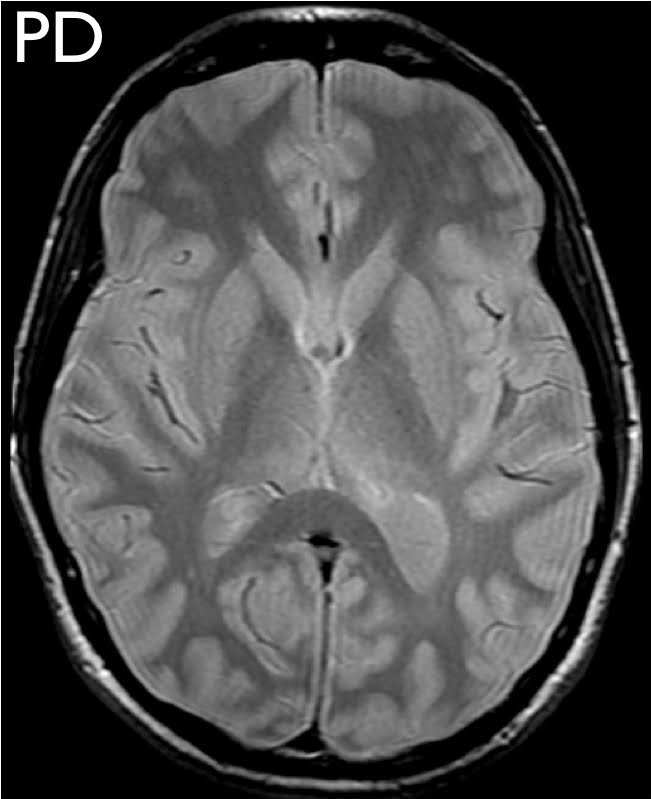
\includegraphics[height=0.6\textheight]{images/pd}

        {\scriptsize Image source: UCSF Dept. of Radiology and Biomedical Imaging}
    \end{columns}
\end{frame}

\begin{frame}{Summary of Common Contrasts}

    \begin{center}
        \begin{tabular}{l||c|c}
            \text{ }          & \textbf{ short TE }            & \textbf{ long TE }            \\ \hline\hline
            \textbf{short TR} & \text{ \longtime{} weighting } & \text{---}                    \\ \hline
            \textbf{long TR}  & \text{ PD weighting }          & \text{\transtime{} weighting}
        \end{tabular}
    \end{center}

    \begin{itemize}
        \item Missing combination:
              \begin{itemize}
                  \item Mixture of \longtime{} and \transtime{} weighting
                  \item No current clinical use
                  \item Weak signal amplitude
              \end{itemize}
    \end{itemize}
\end{frame}

% subsection relaxation_and_contrast (end)

% section nuclear_magnetic_resonance_nmr (end)

\end{document}
